\section{Prototype 3}
\subsection{Algorithm changes}
\subsubsection{Bid and price validation (error fix)}
\begin{figure}[H]
    \centering
    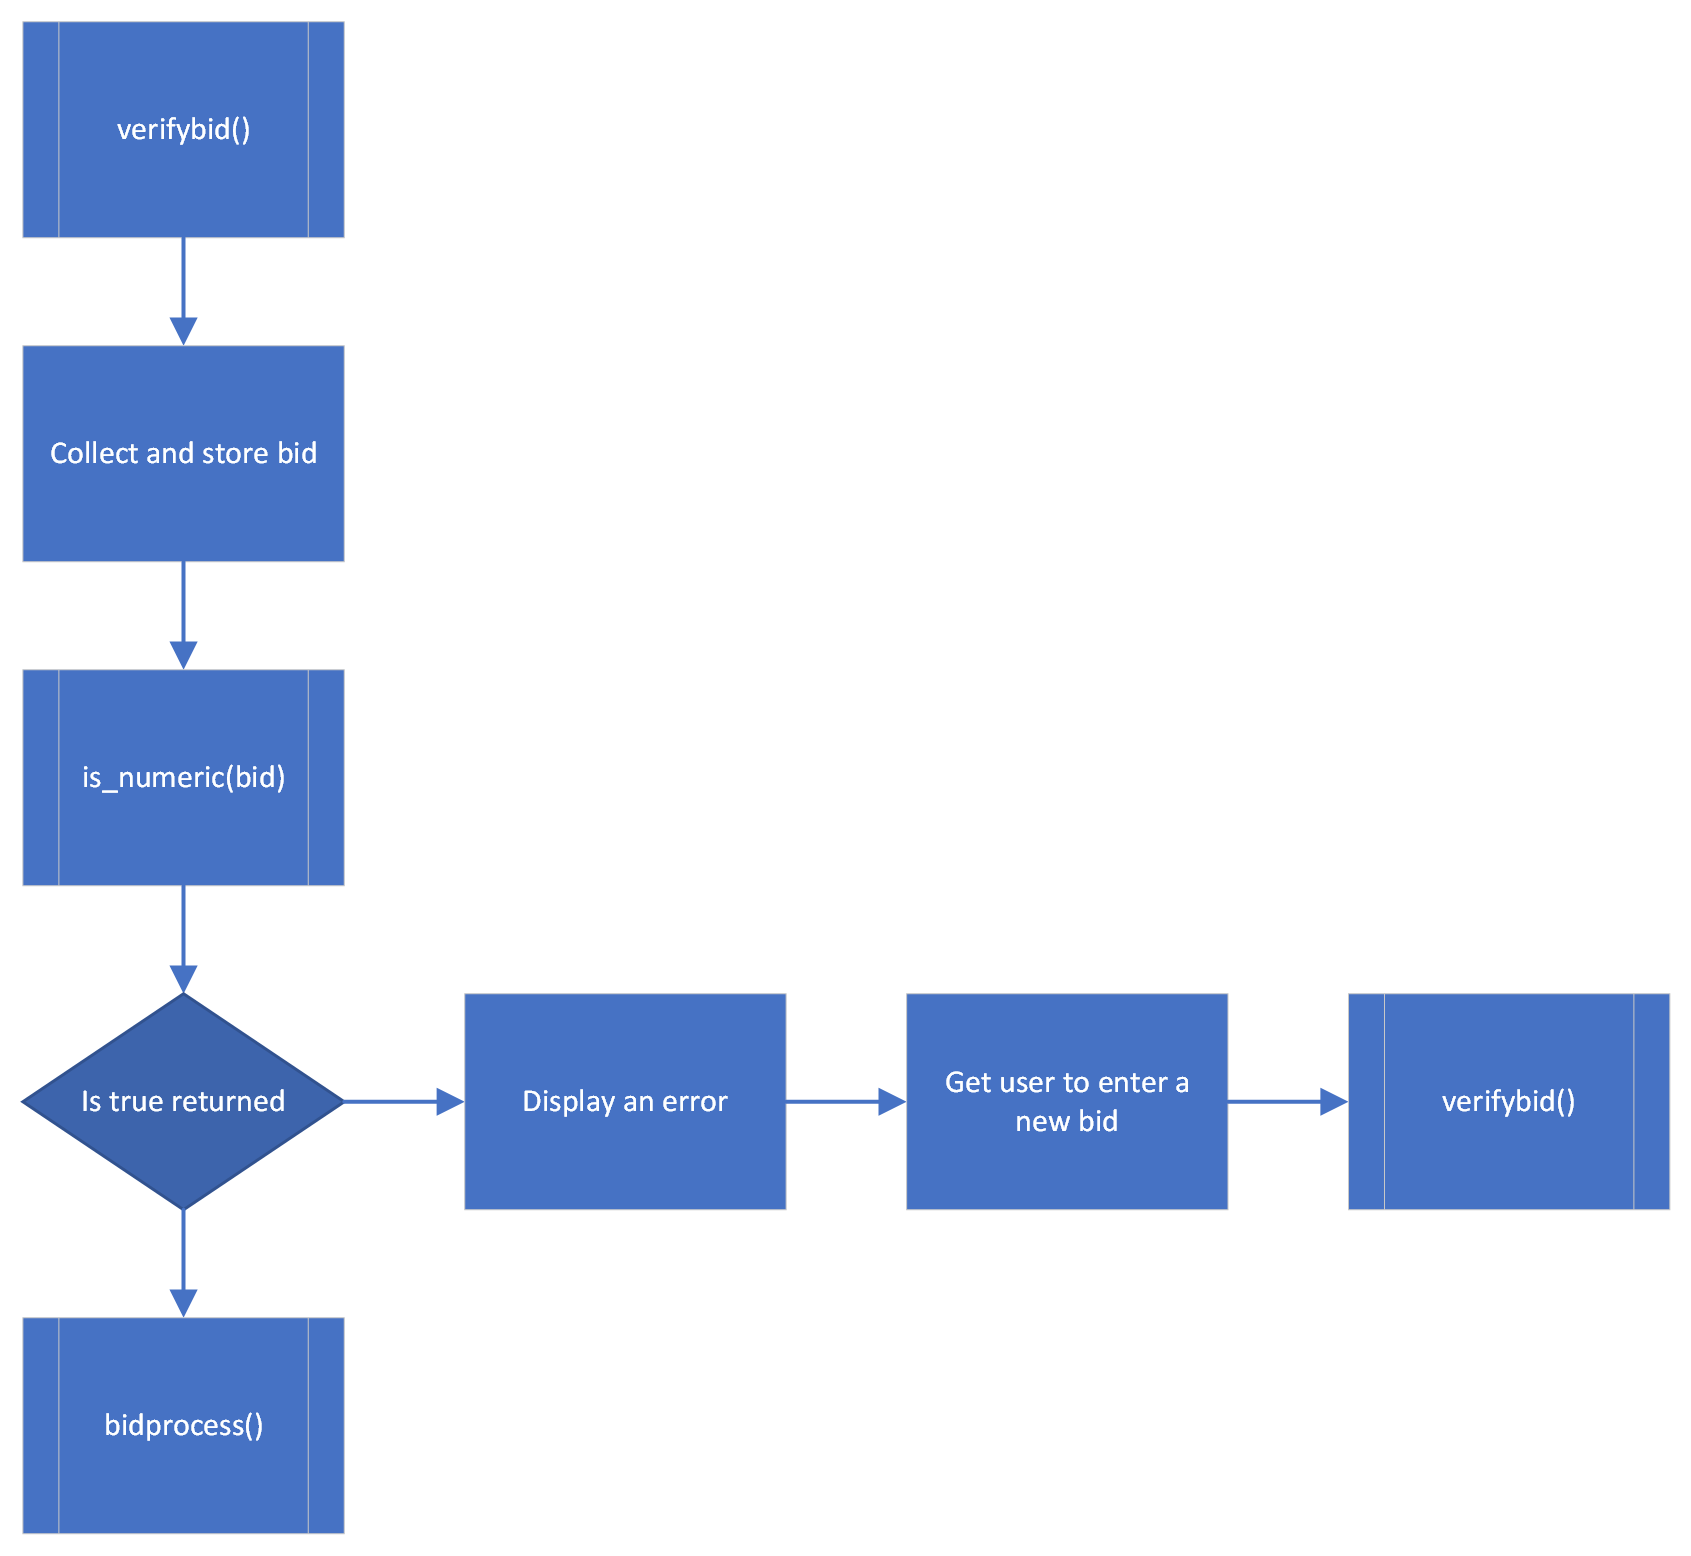
\includegraphics[scale=0.4]{ch3_developing/proto3/flow_bid.png}
    \caption{Prototype 3 new bid validation algorithm flowchart}
    \label{fig:proto3_flowbid}
\end{figure}
 \begin{figure}[H]
     \centering
     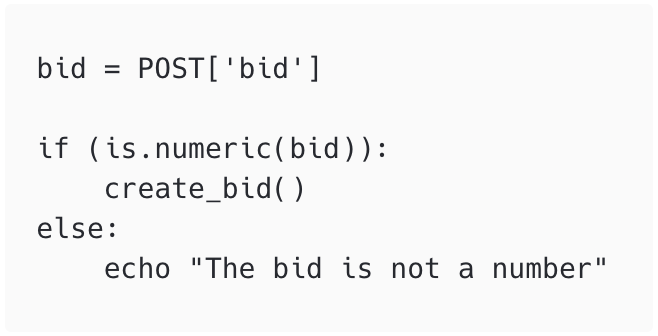
\includegraphics[scale=0.4]{ch3_developing/proto3/bid_integer.png}
     \caption{Prototype 3 new bid validation algorithm pseudocode}
     \label{fig:proto3_bidinteger}
 \end{figure}
 \begin{figure}
     \centering
     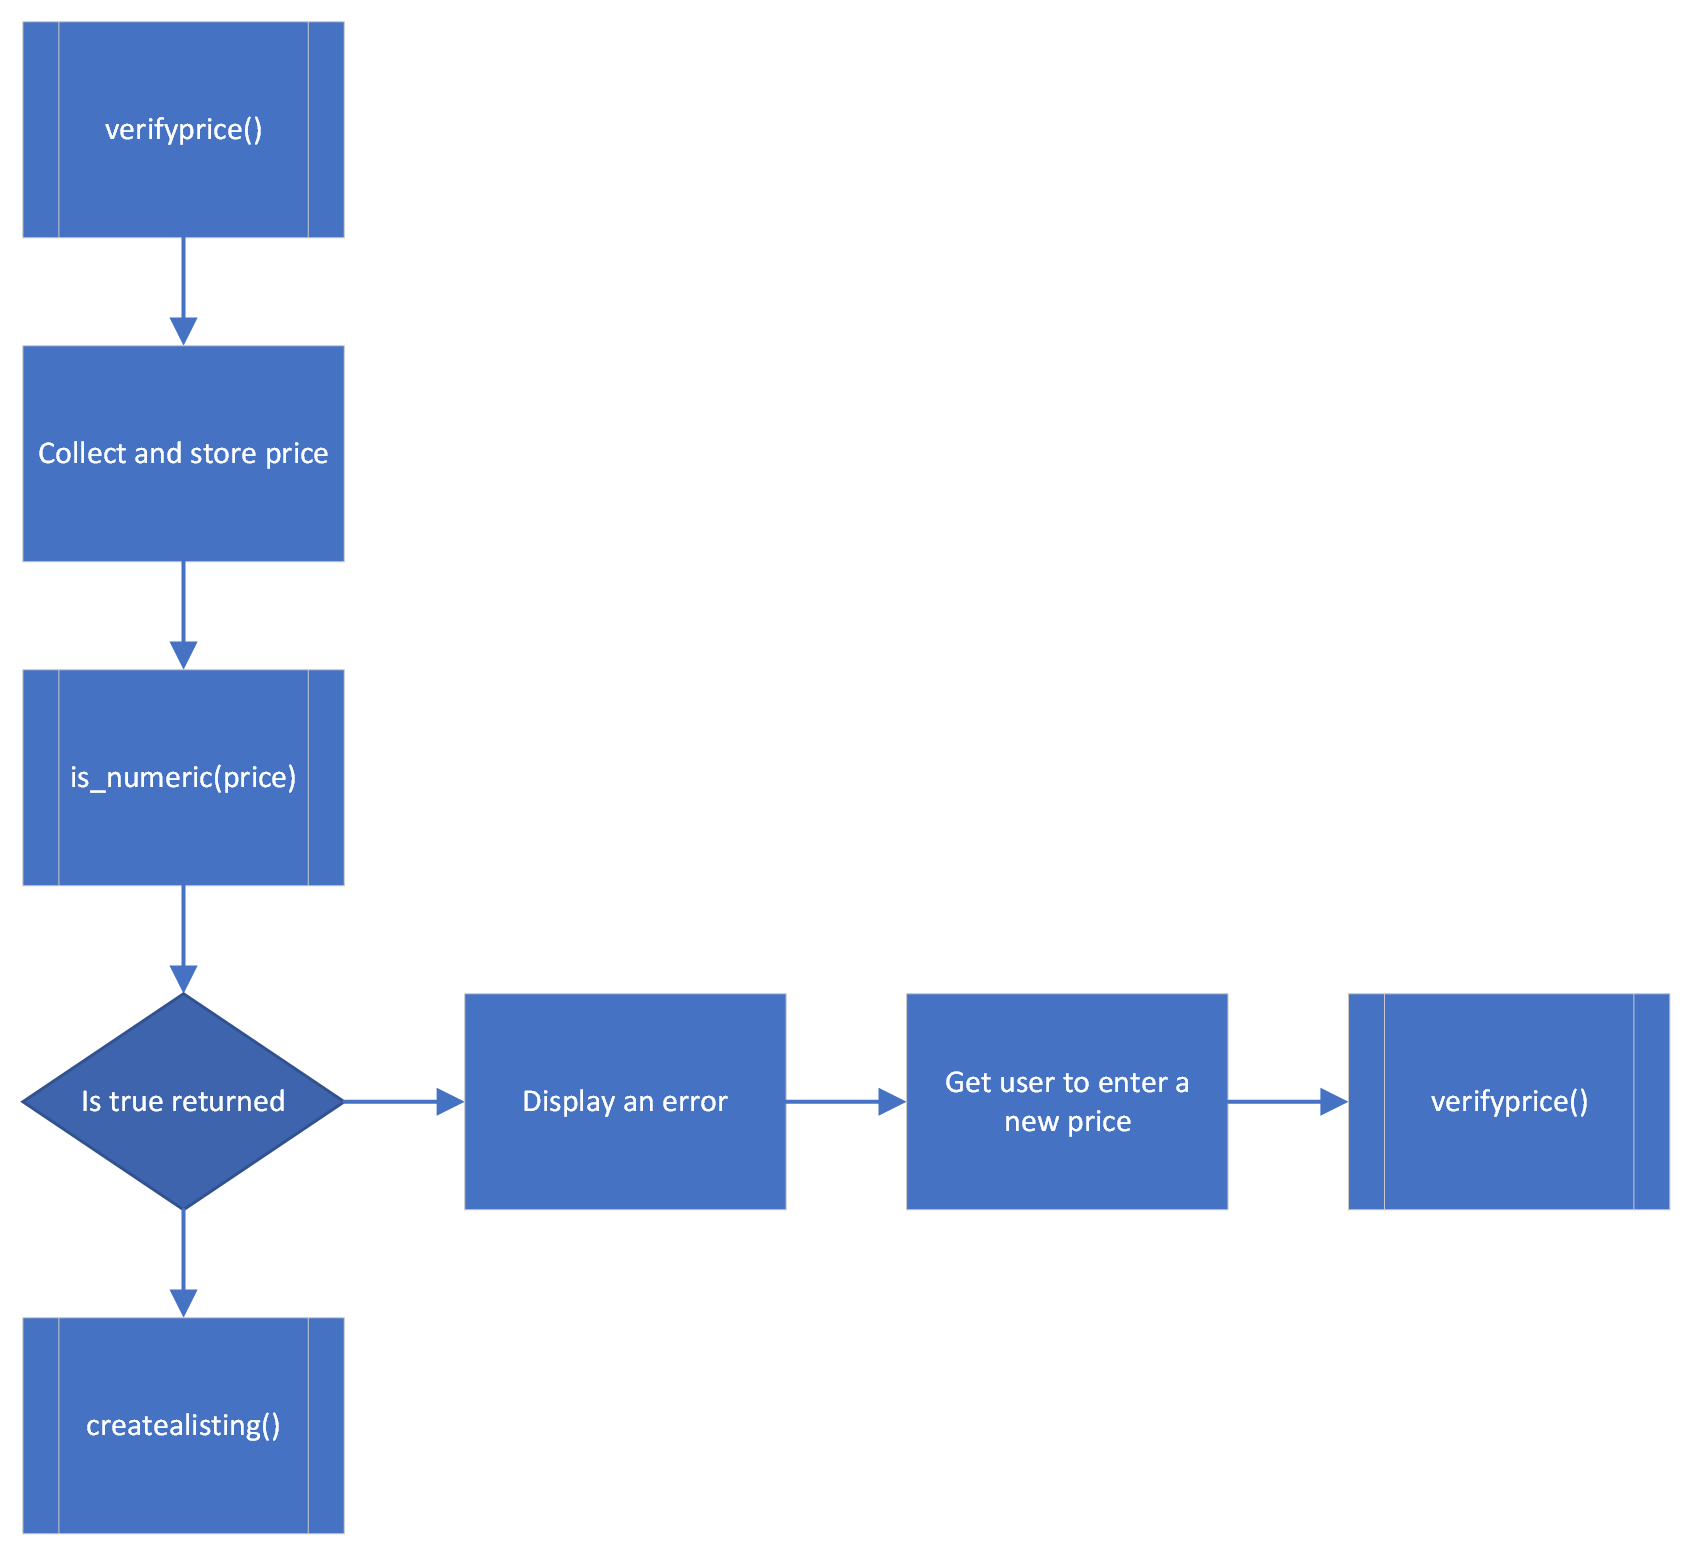
\includegraphics[scale=0.4]{ch3_developing/proto3/flow_price.png}
     \caption{Prototype 3 new price validation algorithm flowchart}
     \label{fig:proto3_flowprice}
 \end{figure}
 \begin{figure}[H]
     \centering
     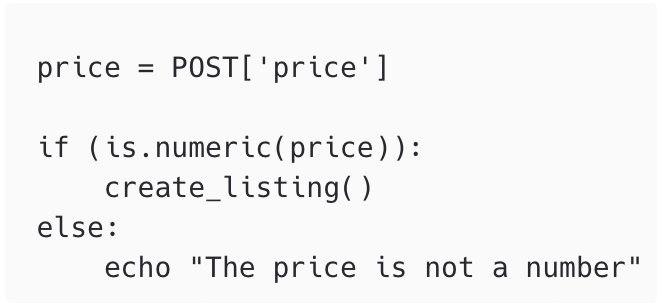
\includegraphics[scale=0.4]{ch3_developing/proto3/price_integer.png}
     \caption{Prototype 3 new price validation algorithm pseudocode}
     \label{fig:proto3_priceinteger}
 \end{figure}
The price and bid algorithms are the same with the changes being for the specific variables and relevant subroutines. They work to first collect the information from the form on the webpage once the user has pressed submit. PHP, where the code will be implemented, has a function built in that can be used for validation so I have used it. The function will return True if the input is a number. The if statement checks to see if true has been returned and if so it will proceed with the relevant subroutine afterwards.

\subsubsection{Image file type validation (error fix)}
\begin{figure}[H]
    \centering
    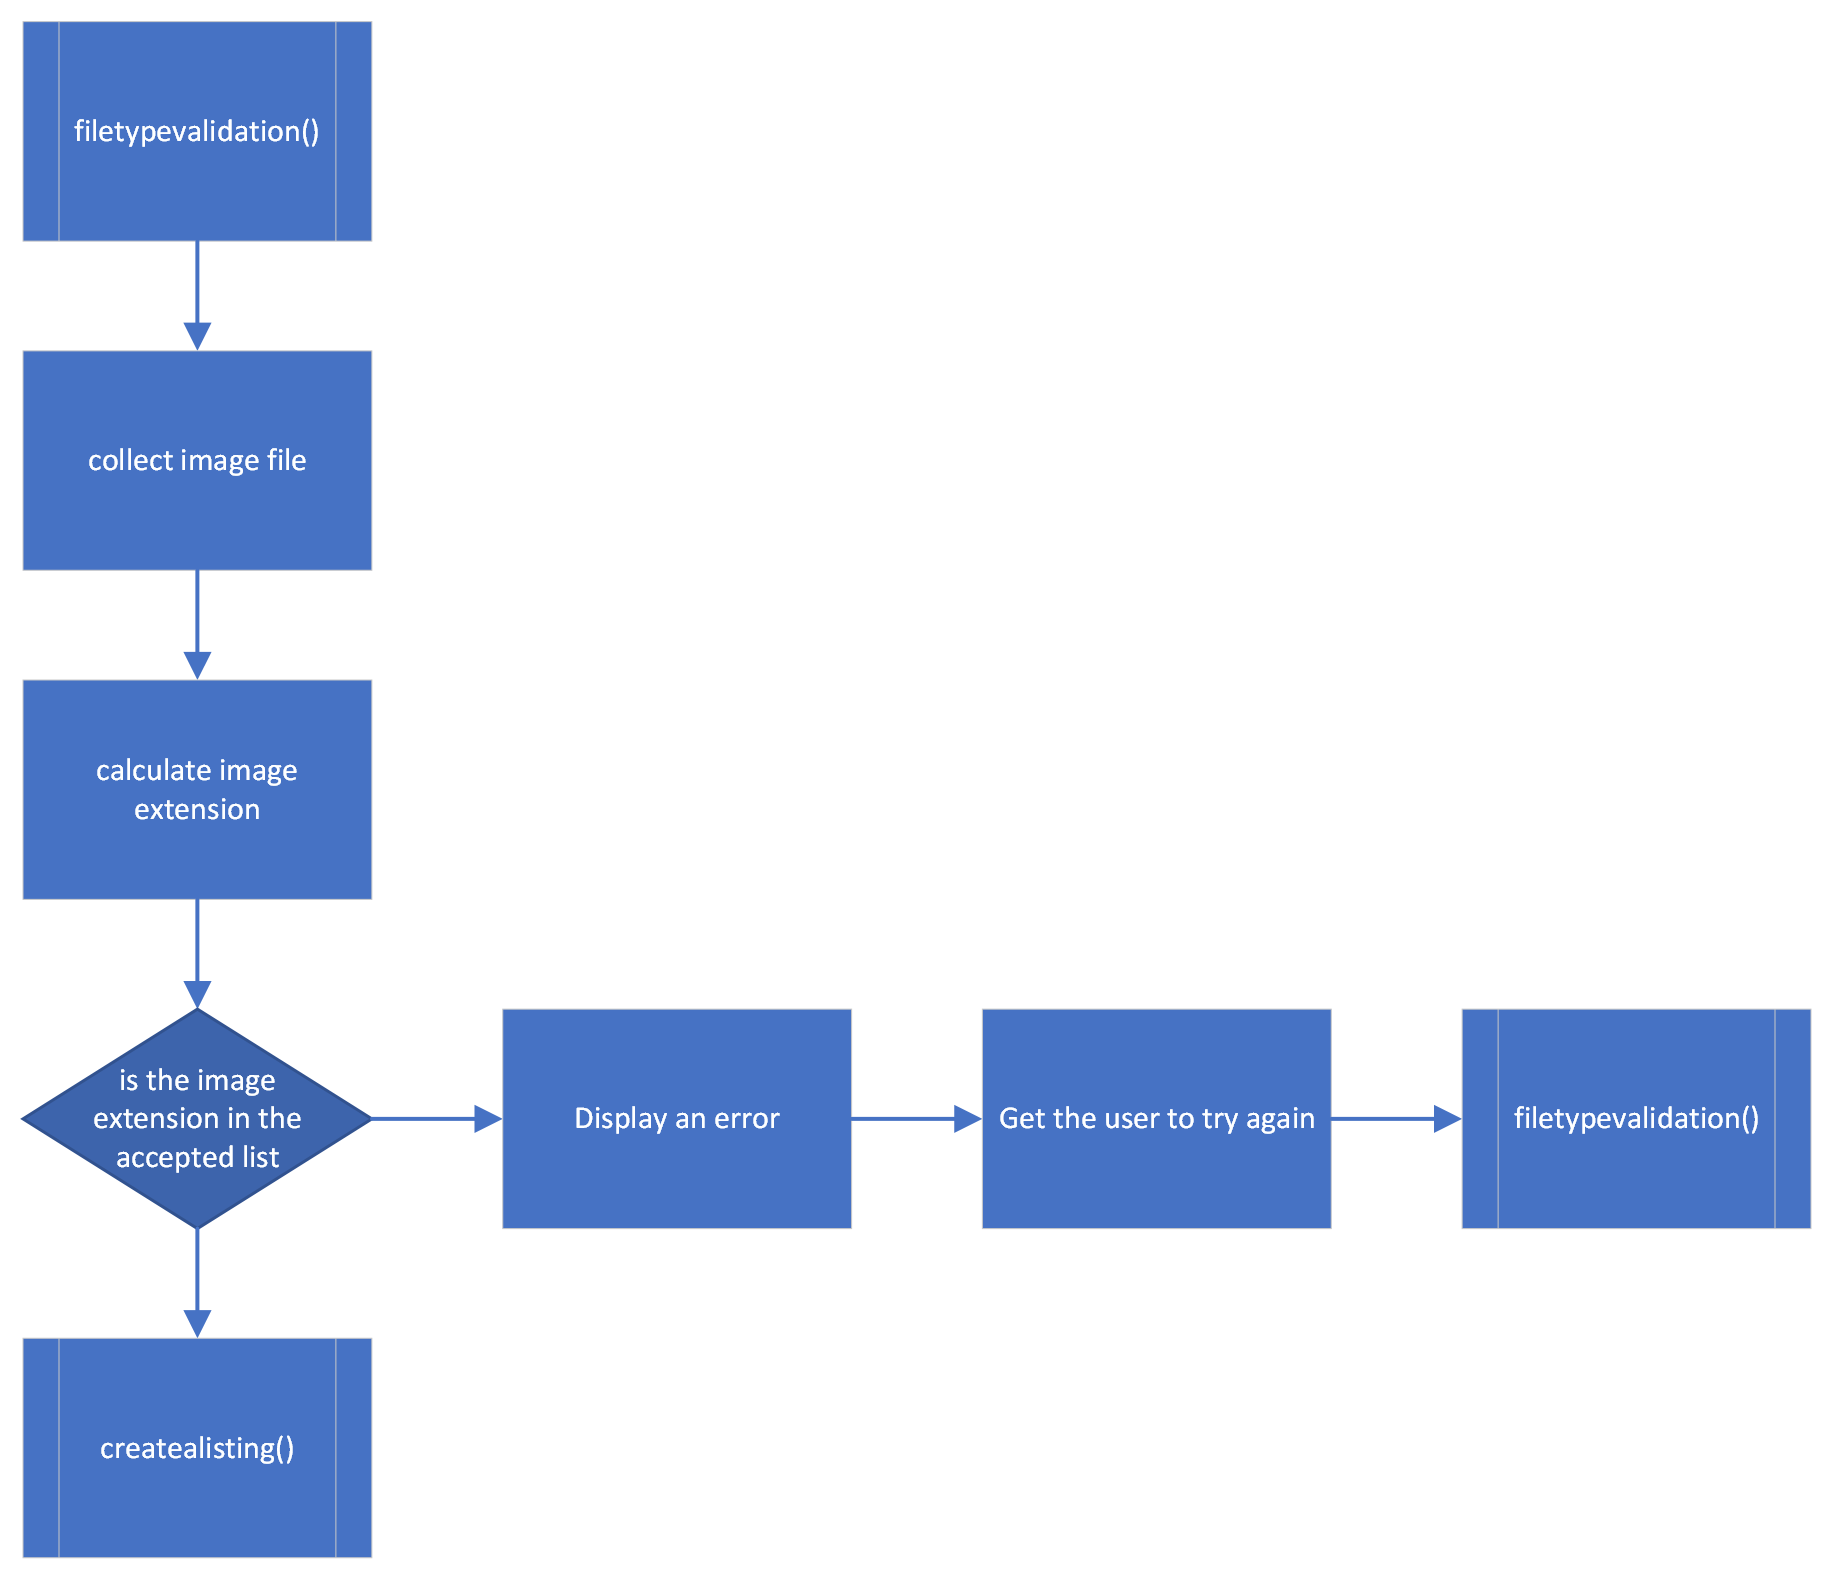
\includegraphics[scale=0.4]{ch3_developing/proto3/flow_imagefile.png}
    \caption{Prototype 3 image validation algorithm flowchart}
    \label{fig:proto3_flowimagefile}
\end{figure}
 \begin{figure}[H]
     \centering
     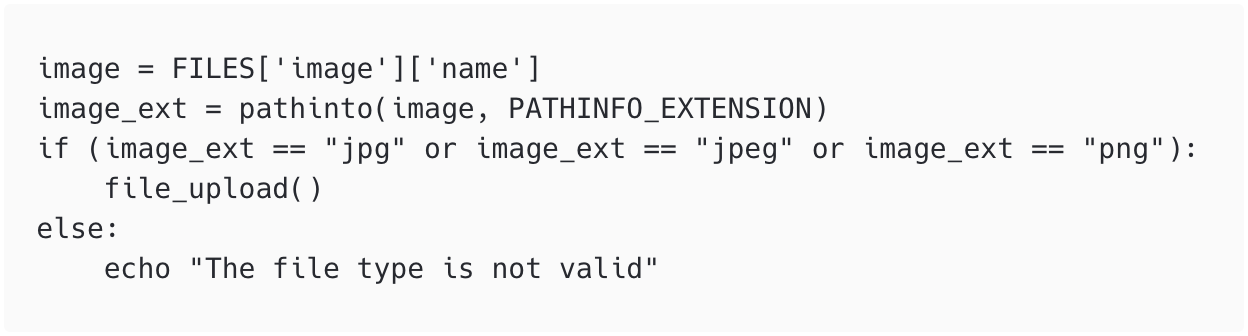
\includegraphics[scale=0.3]{ch3_developing/proto3/image_filetype.png}
     \caption{Prototype 3 image validation algorithm pseudocode}
     \label{fig:proto3_filetypealg}
 \end{figure}
The image is first collected from the upload part of the create a listing. We then assign a variable to just the image extension in order to check it. An if statement is used to check if the file extension is allowed. Multiple comparison statements are used with the or operator allowing any of the file types to be used. Whilst it is not possible to account for every image file extension possible, the 3 chosen: jpg, jpeg and, png are the most common and so will cover the largest quantity of images uploaded to the website. If the file extension is valid, the file\_upload() function can run which will upload the image file to the correct folder on the server. If the image extension is not valid, then we show the user a specific error to tell them that the file type is causing an issue in creating the listing.  

\subsubsection{Registration hashing (new feature)}
 \begin{figure}[H]
    \centering
    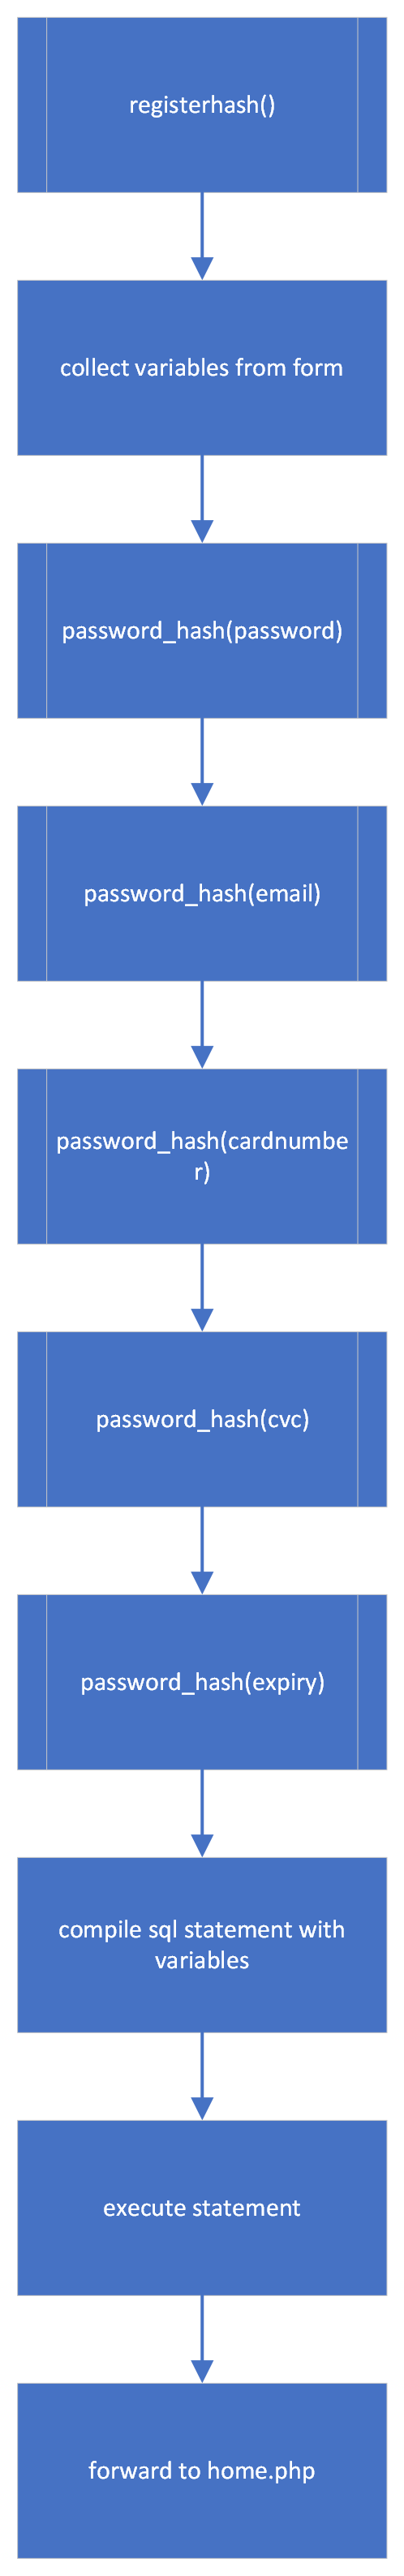
\includegraphics[scale=0.4]{ch3_developing/proto3/flow_register.png}
    \caption{Prototype 3 registration hashing flowchart}
    \label{fig:proto3_hashingflow}
\end{figure}
 \begin{figure}[H]
     \centering
     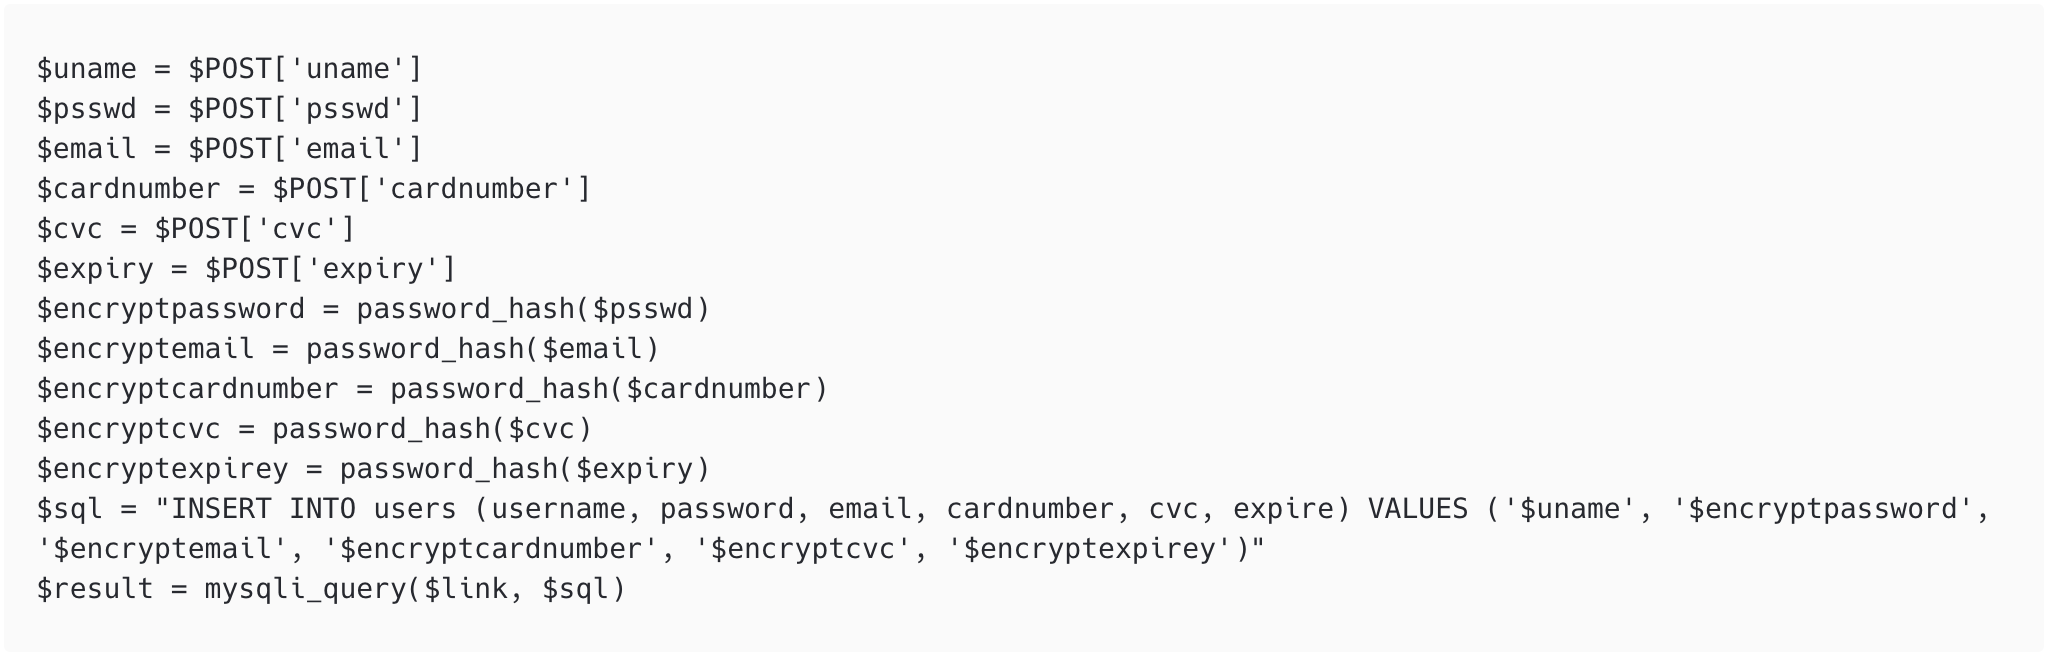
\includegraphics[scale=0.2]{ch3_developing/proto3/register_hash.png}
     \caption{Prototype 3 registration hashing pseudocode}
     \label{fig:proto3_hasingalg}
 \end{figure}
The algorithm works to first collect all the information from the registration form. Using the PHP hashing function, we hash all variables which need to be kept secure. The decision was taken to not hash the username since it is used as an identifier and is displayed to the user. Displaying the username when it has been hashed would cause issues for pages such as the messages page.  Once all the values have been hashed, they are added to an SQL statement which is then executed and thus creates the users account for the website. 
\subsubsection{Sending message (new feature)}
  \begin{figure}[H]
    \centering
    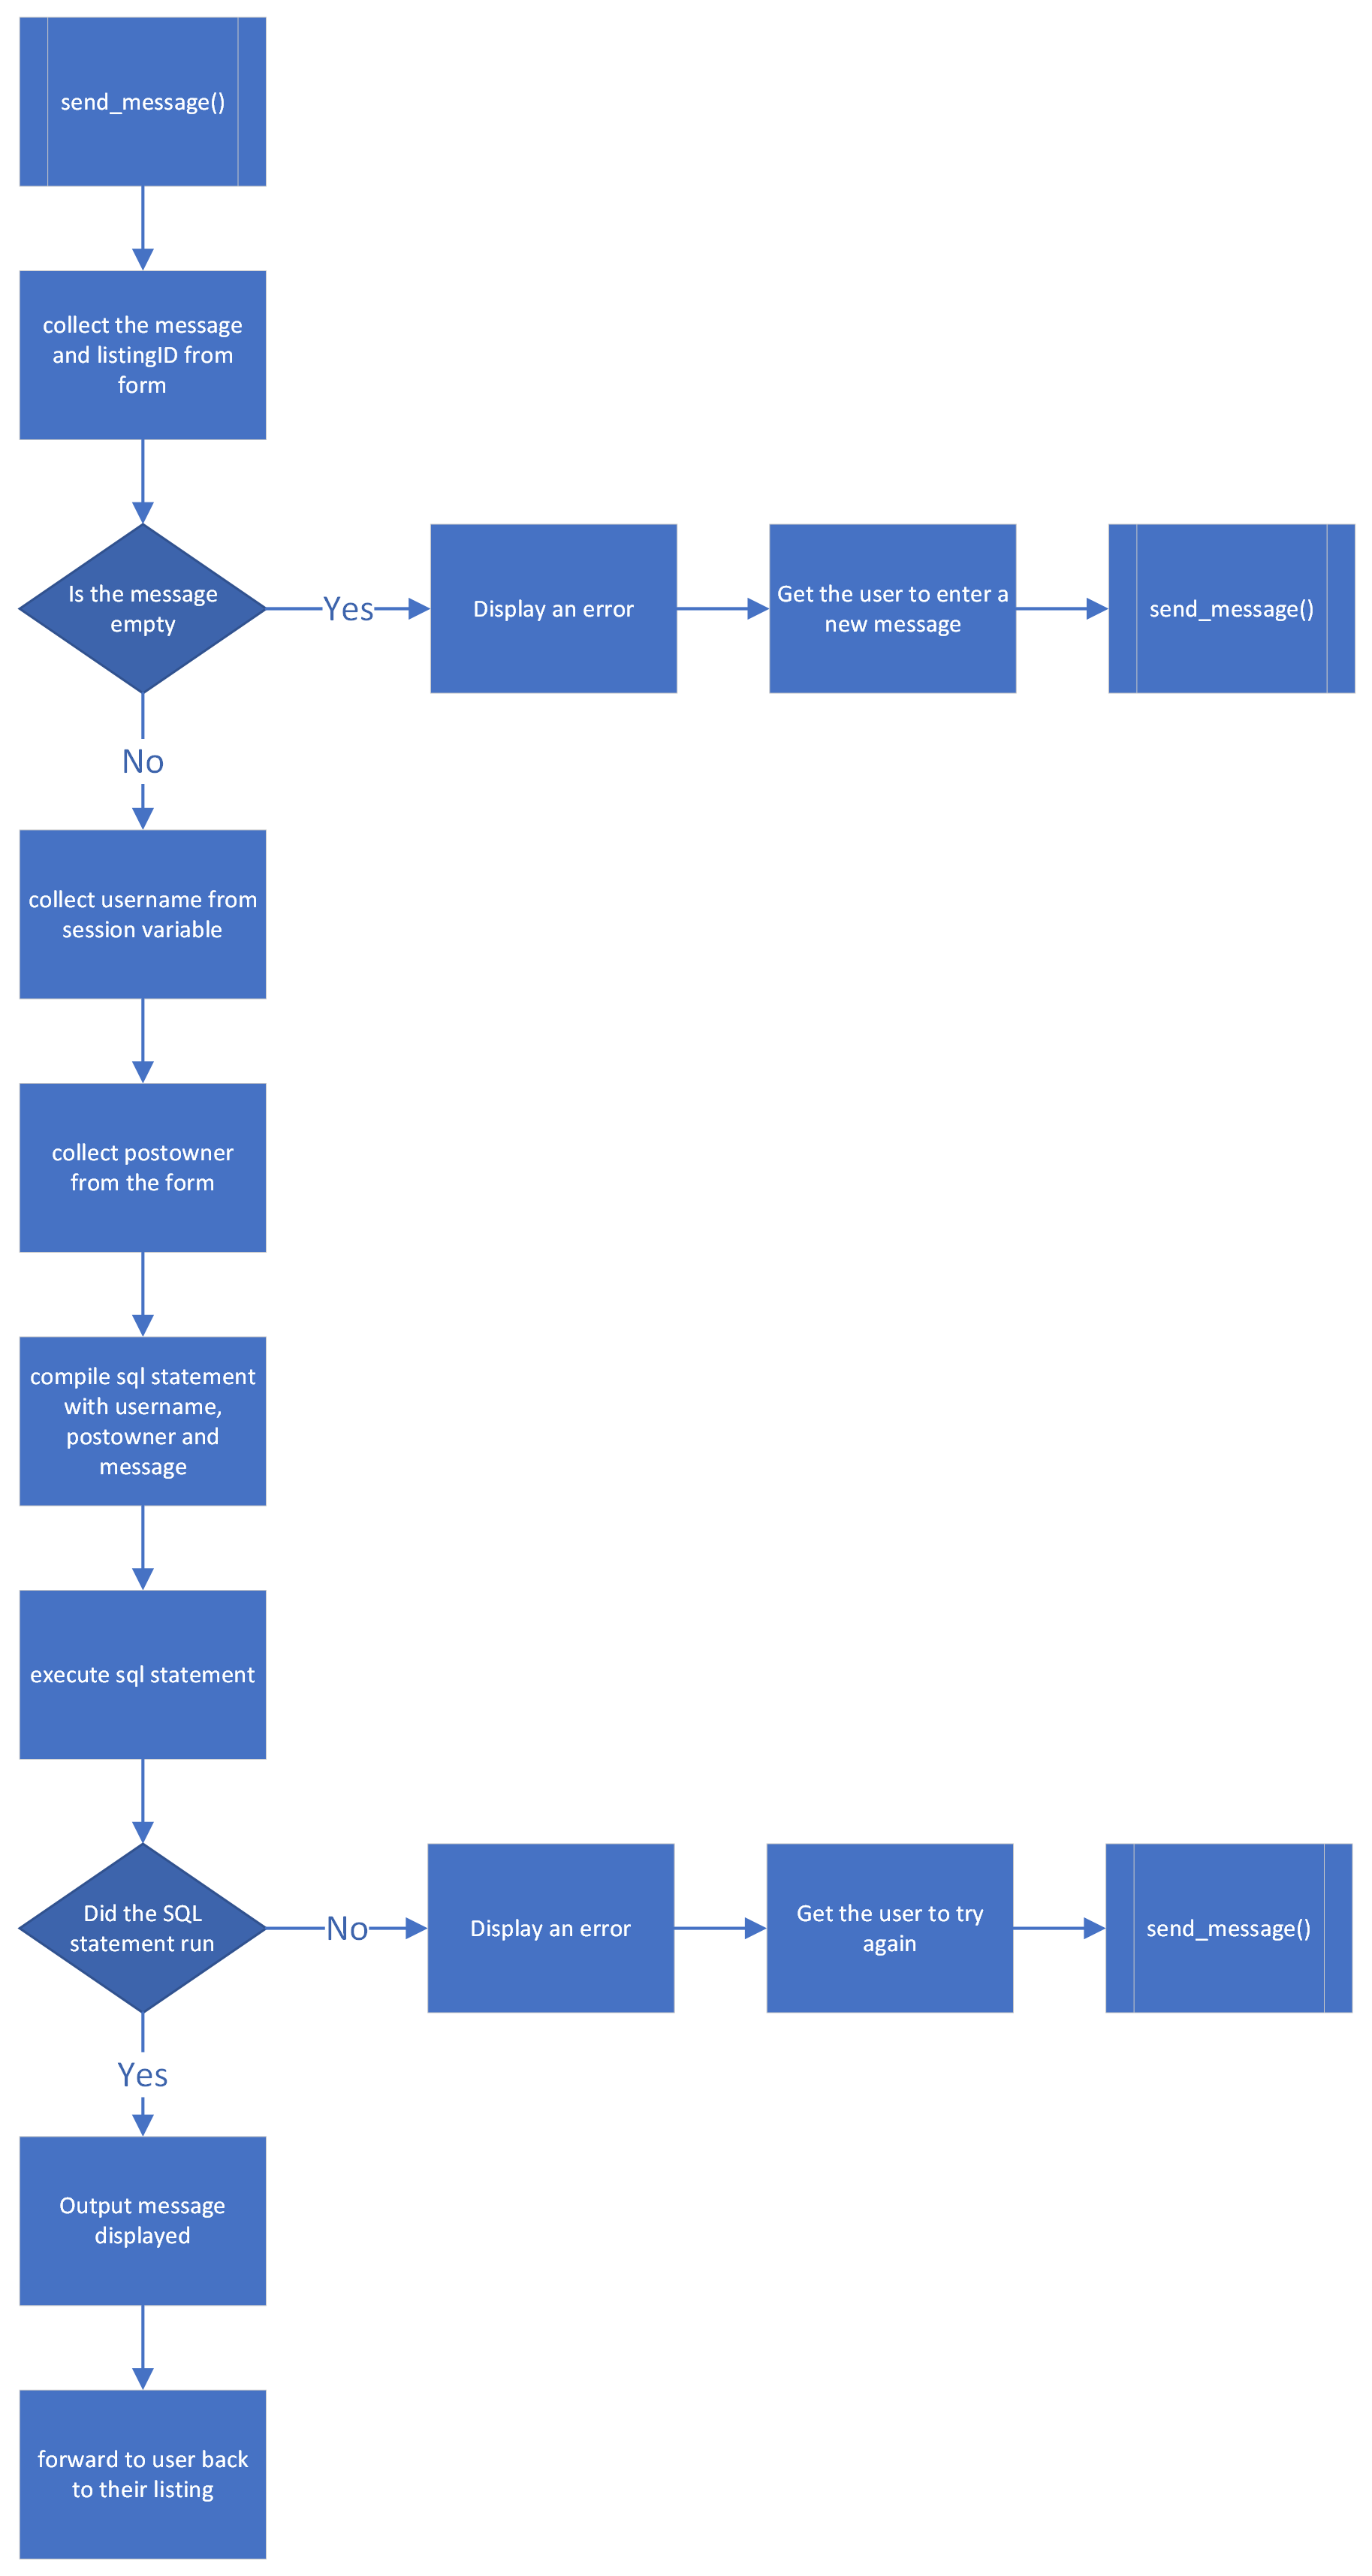
\includegraphics[scale=0.4]{ch3_developing/proto3/flow_sendmessage.png}
    \caption{Prototype 3 send message flowchart}
    \label{fig:proto3_sendflow}
\end{figure}
 \begin{figure}[H]
     \centering
     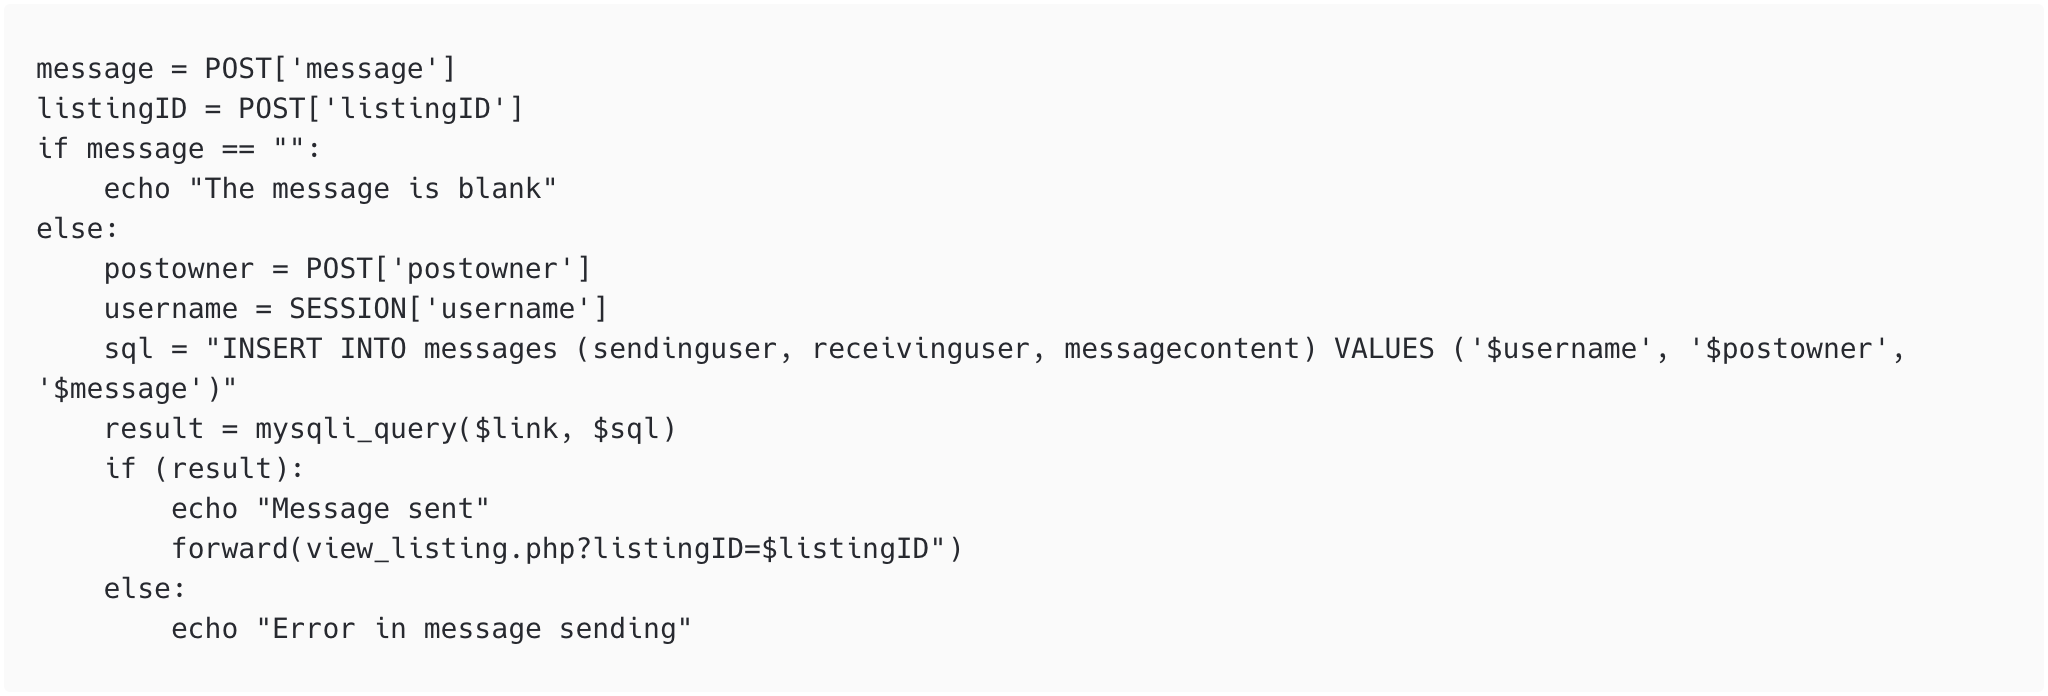
\includegraphics[scale=0.2]{ch3_developing/proto3/message_send.png}
     \caption{Prototype 3 send message pseudocode}
     \label{fig:proto3_sendalg}
 \end{figure} 
The code will first work to collect the users listingsID and message from the form. The message is then checked using an if statement to see if it is blank. If the message is blank, then we send the user an error. Else, the postowner is collected and the username retrieved from a session variable. This is so that we know who the message is to and who it is from. The SQL statement is then queried to send the message to the database. If the result is executed without an error the user is sent back to their listing. If not, they are given an error message telling them there was an error in sending. 

\subsubsection{Receive message (new feature)}
\begin{figure}[H]
    \centering
    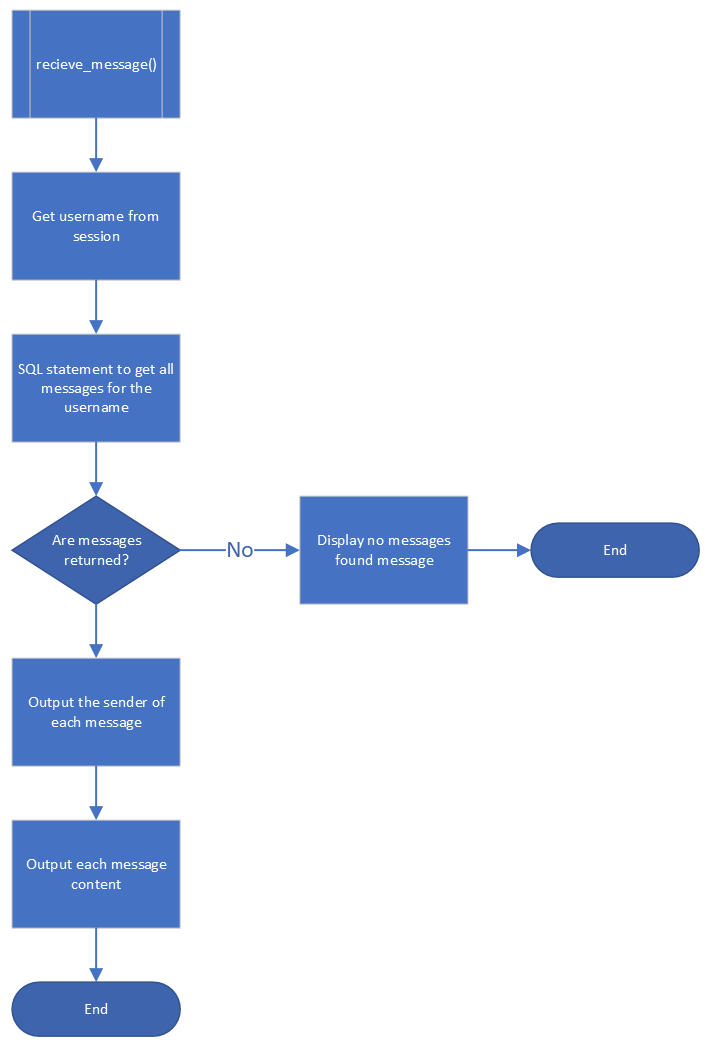
\includegraphics[scale=0.5]{ch3_developing/proto3/flow_recievemessage.png}
    \caption{Prototype 3 receive message flowchart}
    \label{fig:proto3_registerflow}
\end{figure}
 \begin{figure}[H]
     \centering
     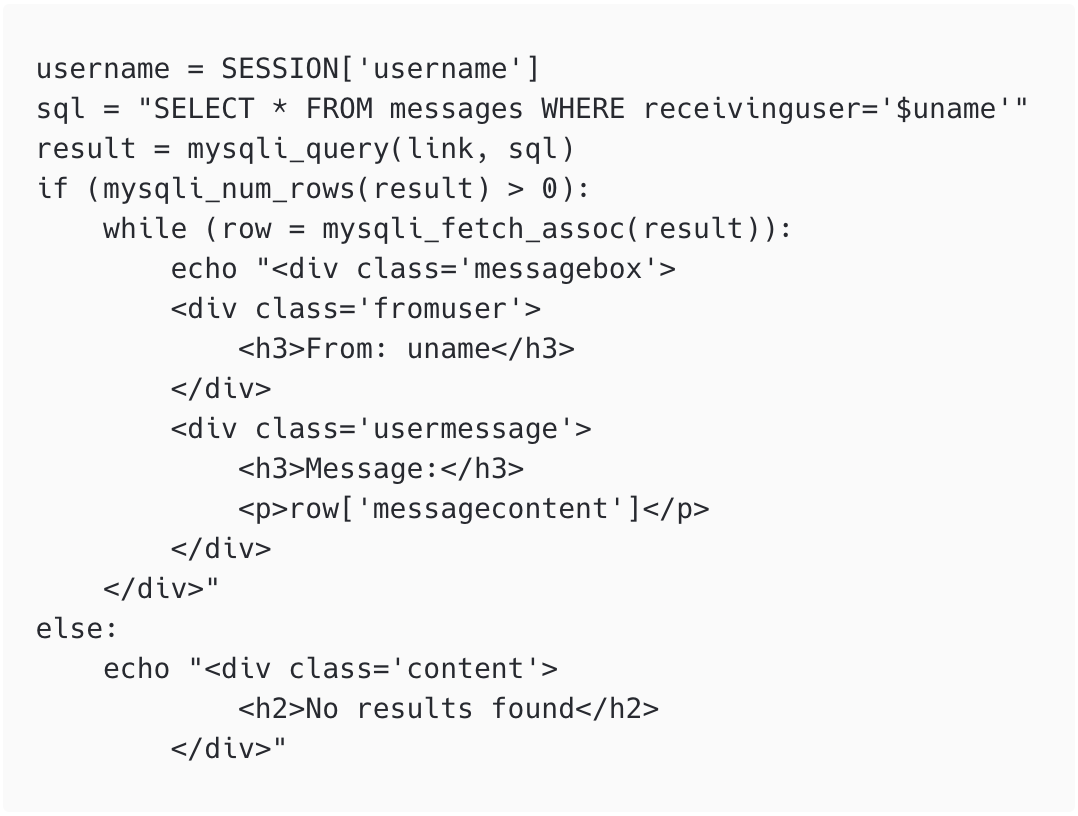
\includegraphics[scale=0.4]{ch3_developing/proto3/message_recieve.png}
     \caption{Prototype 3 receive message pseudocode}
     \label{fig:proto3_registeralg}
 \end{figure} 
In order to collect the listings, we just need to know the user’s username. To do this, we collect it from the session variable. We then use an SQL statement to query the database where we look for the receivinguser column to equal the username. If results are returned, we output each one through a while loop. Each message is outputted with the HTML required to format the appearance of the messages. If no results are found then we output an error message. 

\subsection{Login code}
\begin{figure}[H]
    \centering
    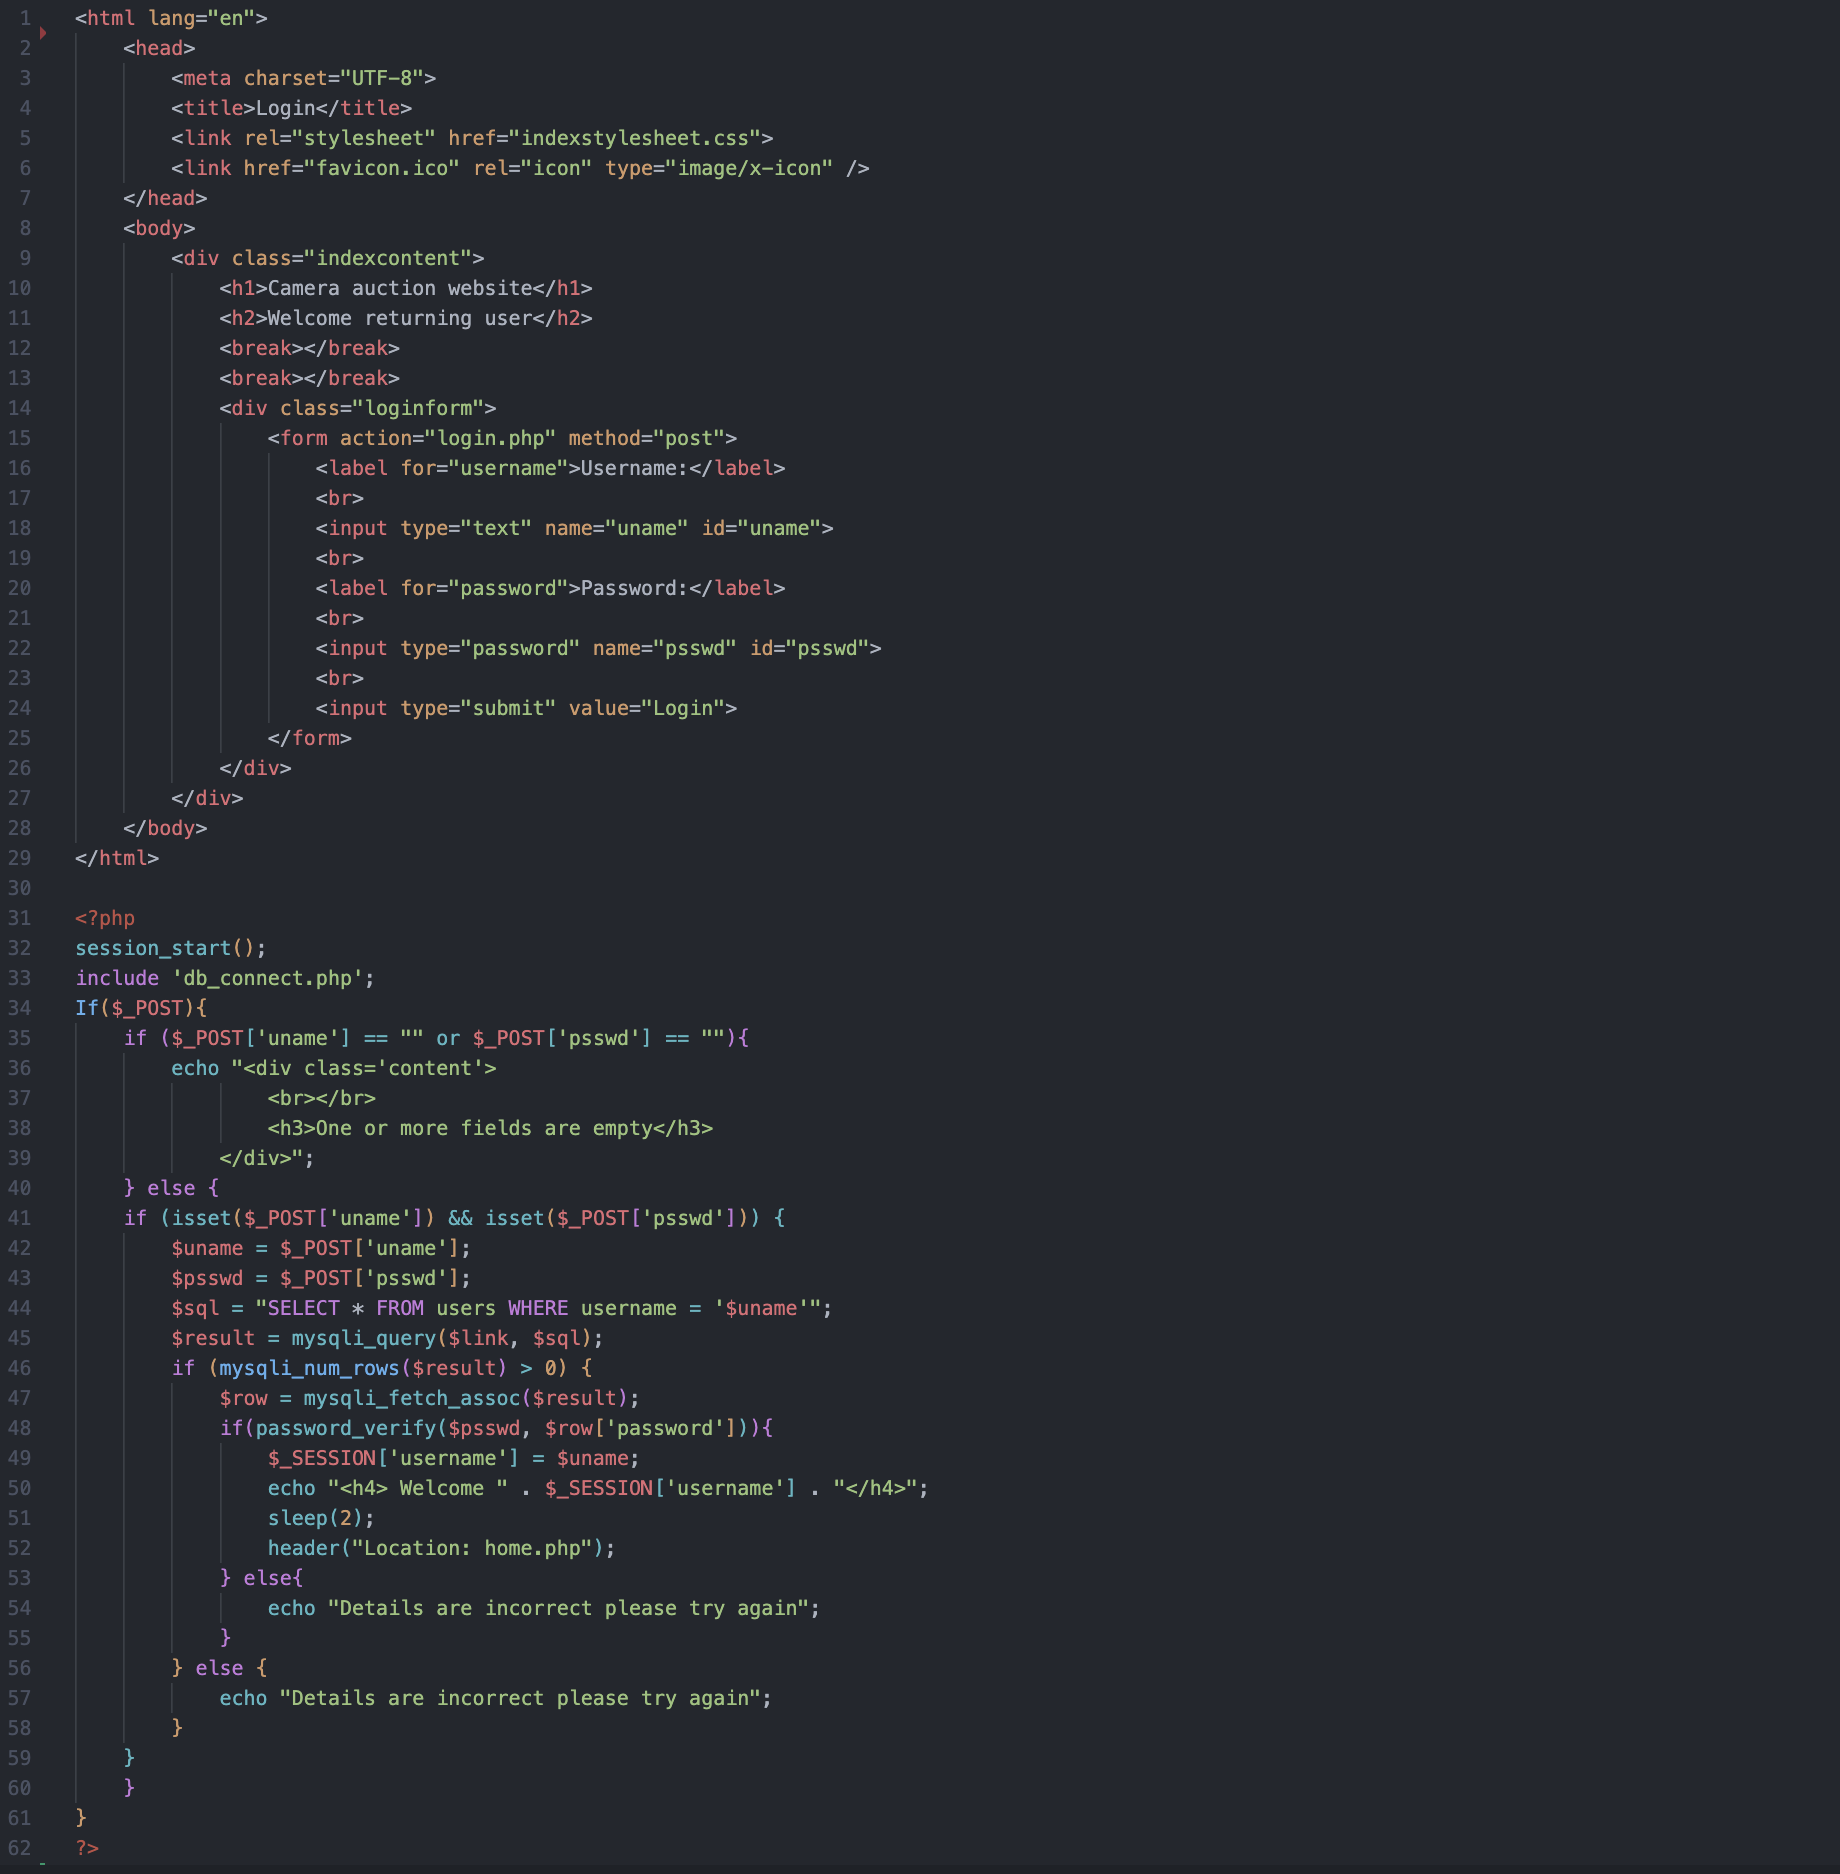
\includegraphics[scale=0.5]{ch3_developing/proto3/login.png}
    \caption{Prototype 3 Login code}
    \label{fig:proto3_login}
\end{figure}
The login algorithm has been updated so to include and account for the hashing of the user’s password. The box is first checked that it contains text in it to ensure that the user cannot just bypass the login. The variables are the then collected with all of the user’s data being fetched using the username. This is to ensure that we can session the username variable or can use the card details later on in the website. The password has previously been hashed and so the password\_verify() function in PHP has to be used to check that the passwords match. Providing that the passwords match, the user if forwarded onto the home page and the username is added to a session variable as it will be used later on. 
\subsection{Sign-up code}
\begin{figure}[H]
    \centering
    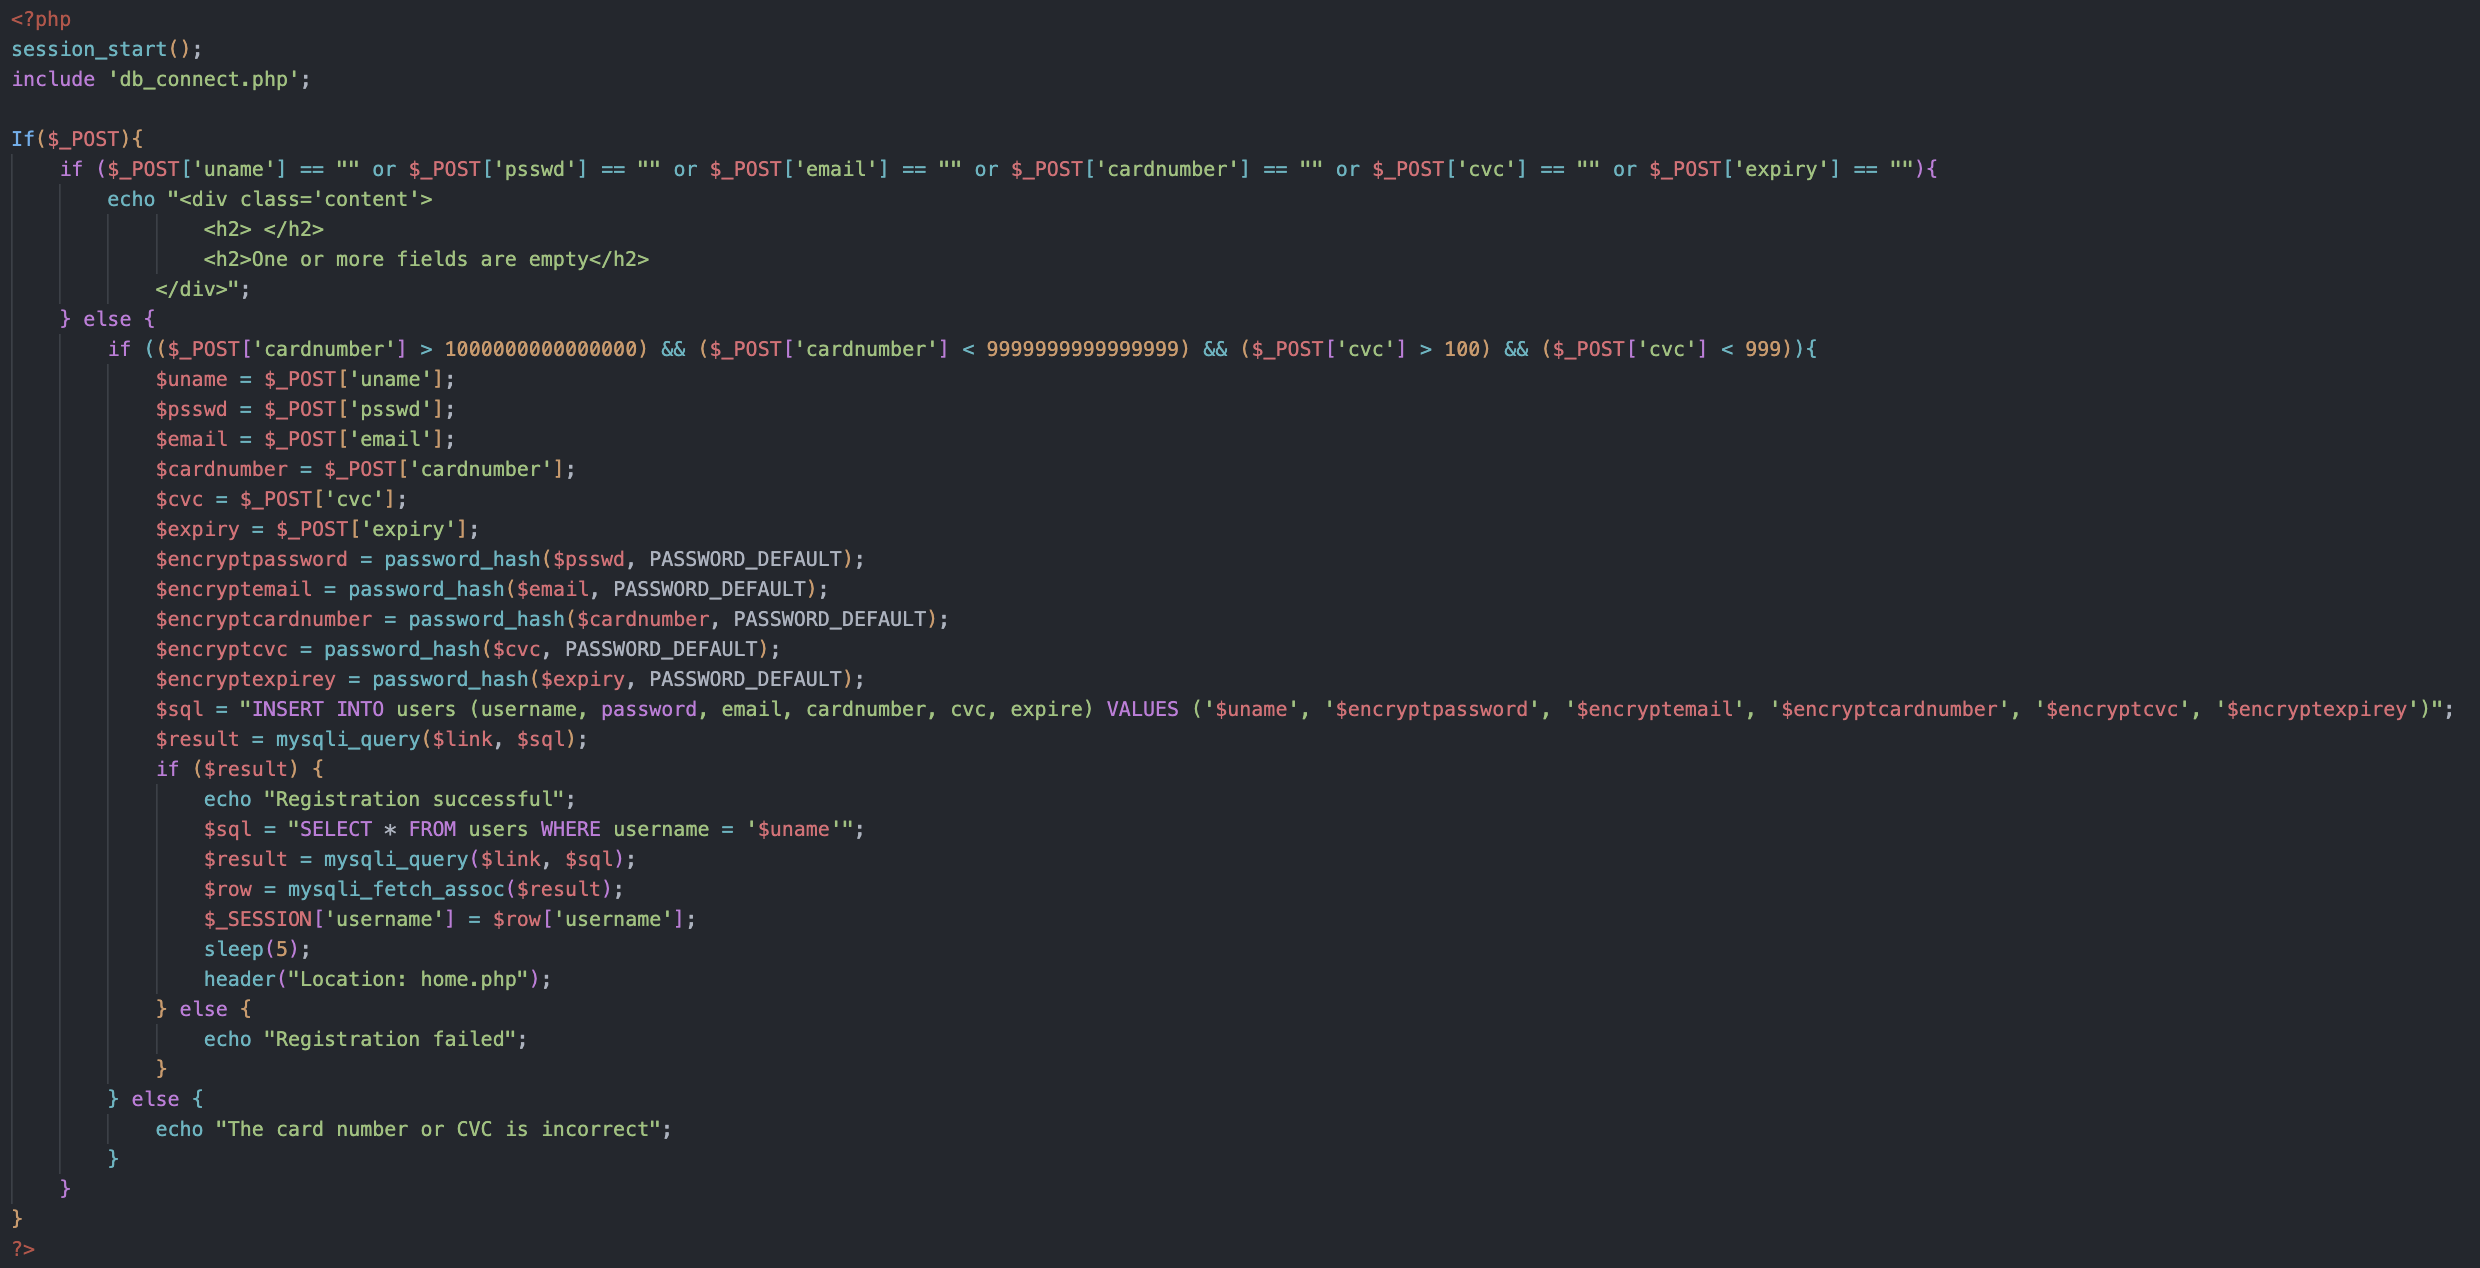
\includegraphics[scale=0.35]{ch3_developing/proto3/register.png}
    \caption{Prototype 3 Registration code}
    \label{fig:proto3_register}
\end{figure}
The sign-up code has had to the addition of hashing all of the user’s important details. This was aimed to better ensure the security of the website and mean that if someone got access to the database, they could not steal any data. This was achieved through PHP’s password\_hash() function. Providing that all the boxes have text in them, they are each hash with the hash value being assigned to a new variable. Since the username is needed for the running of the site, I choose not to hash it. All the encrypted values are added into SQL statement which is then executed. The user’s username is then also assigned to a session variable similar to the login code in order to ensure the running of the website. The user is then forwarded to the home page.
\subsection{Home page}
\begin{figure}[H]
    \centering
    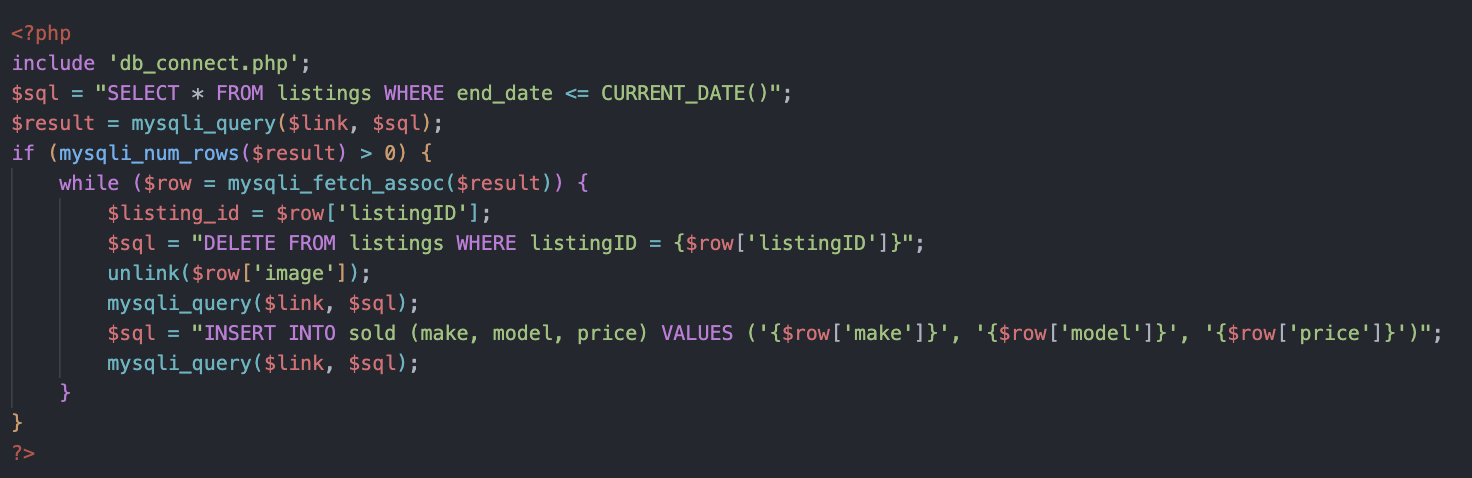
\includegraphics[scale=0.5]{ch3_developing/proto3/home.png}
    \caption{Prototype 3 home page}
    \label{fig:proto3_home}
\end{figure}
The home page contains the code to delete and remove the listings that are out of date. I chose to put the code on this page since it is the most frequently accessed and so would mean that more updates are being sent to the database. This would mean that if a listing had just ended, it would be removed as quickly as possible due to the frequency of traffic to the home page. The listings are first found that are out of time. A while loop cycles through them, first deleting it from the sites current listings and into the sold database. The image is then removed from the server. Only the make, model and sold prices are added to the database since that is all that is needed for the recommended price algorithm. 
\subsection{Search code}
 \begin{figure}[H]
    \centering
    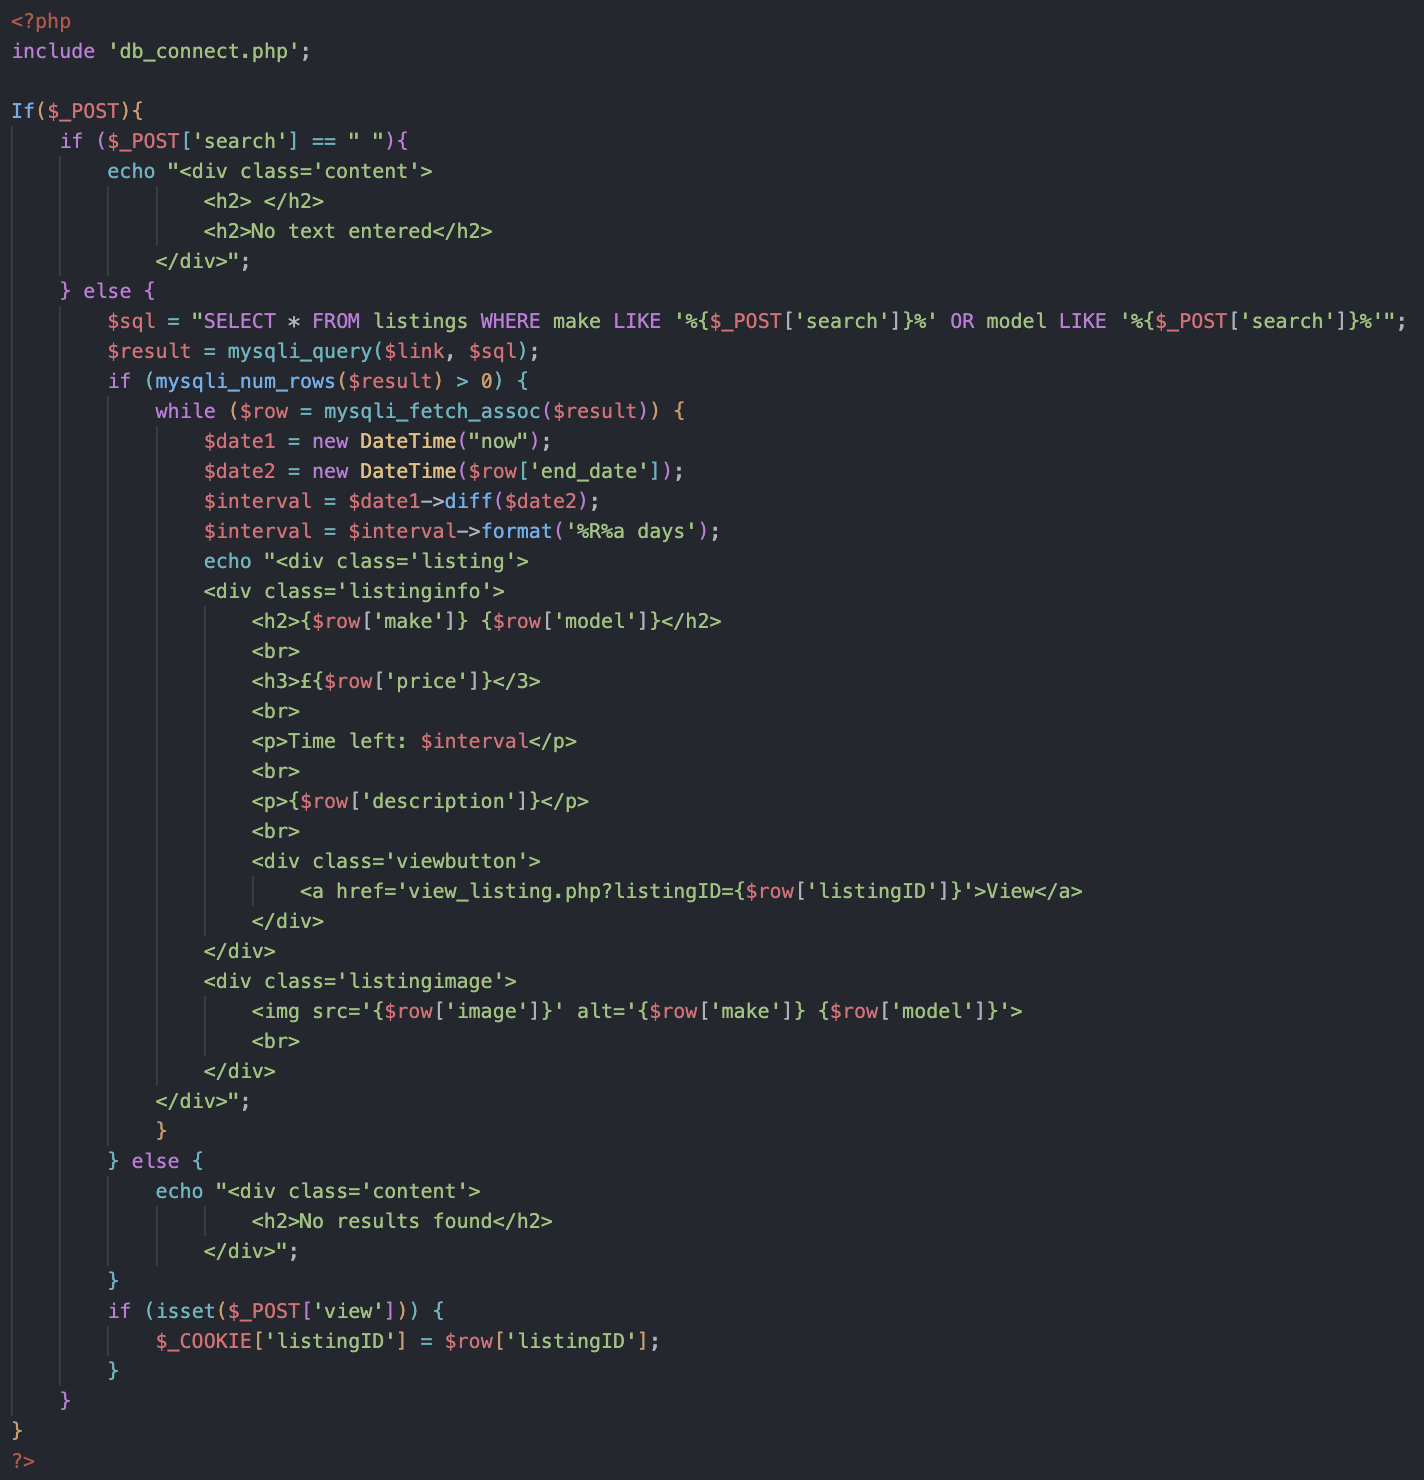
\includegraphics[scale=0.5]{ch3_developing/proto3/search.png}
    \caption{Prototype 3 search page}
    \label{fig:proto3_search}
\end{figure}
The search code will use the term from the users search to query both the make and model columns to best increase the chance of being able to find a listing that they want. If any listings are returned, they are cycled through with a while loop. The time left on each listing is calculated to better show the user how much time is left rather than just the data at which the listing will end. Each listing is then echoed the user alongside the relevant html in order to ensure styling is correct. If no listing is found, then the user is shown an error message. If the user chooses to view a listing, the listingID is passed through to the page as a request. 
\subsection{Create a listing code}
\begin{figure}[H]
    \centering
    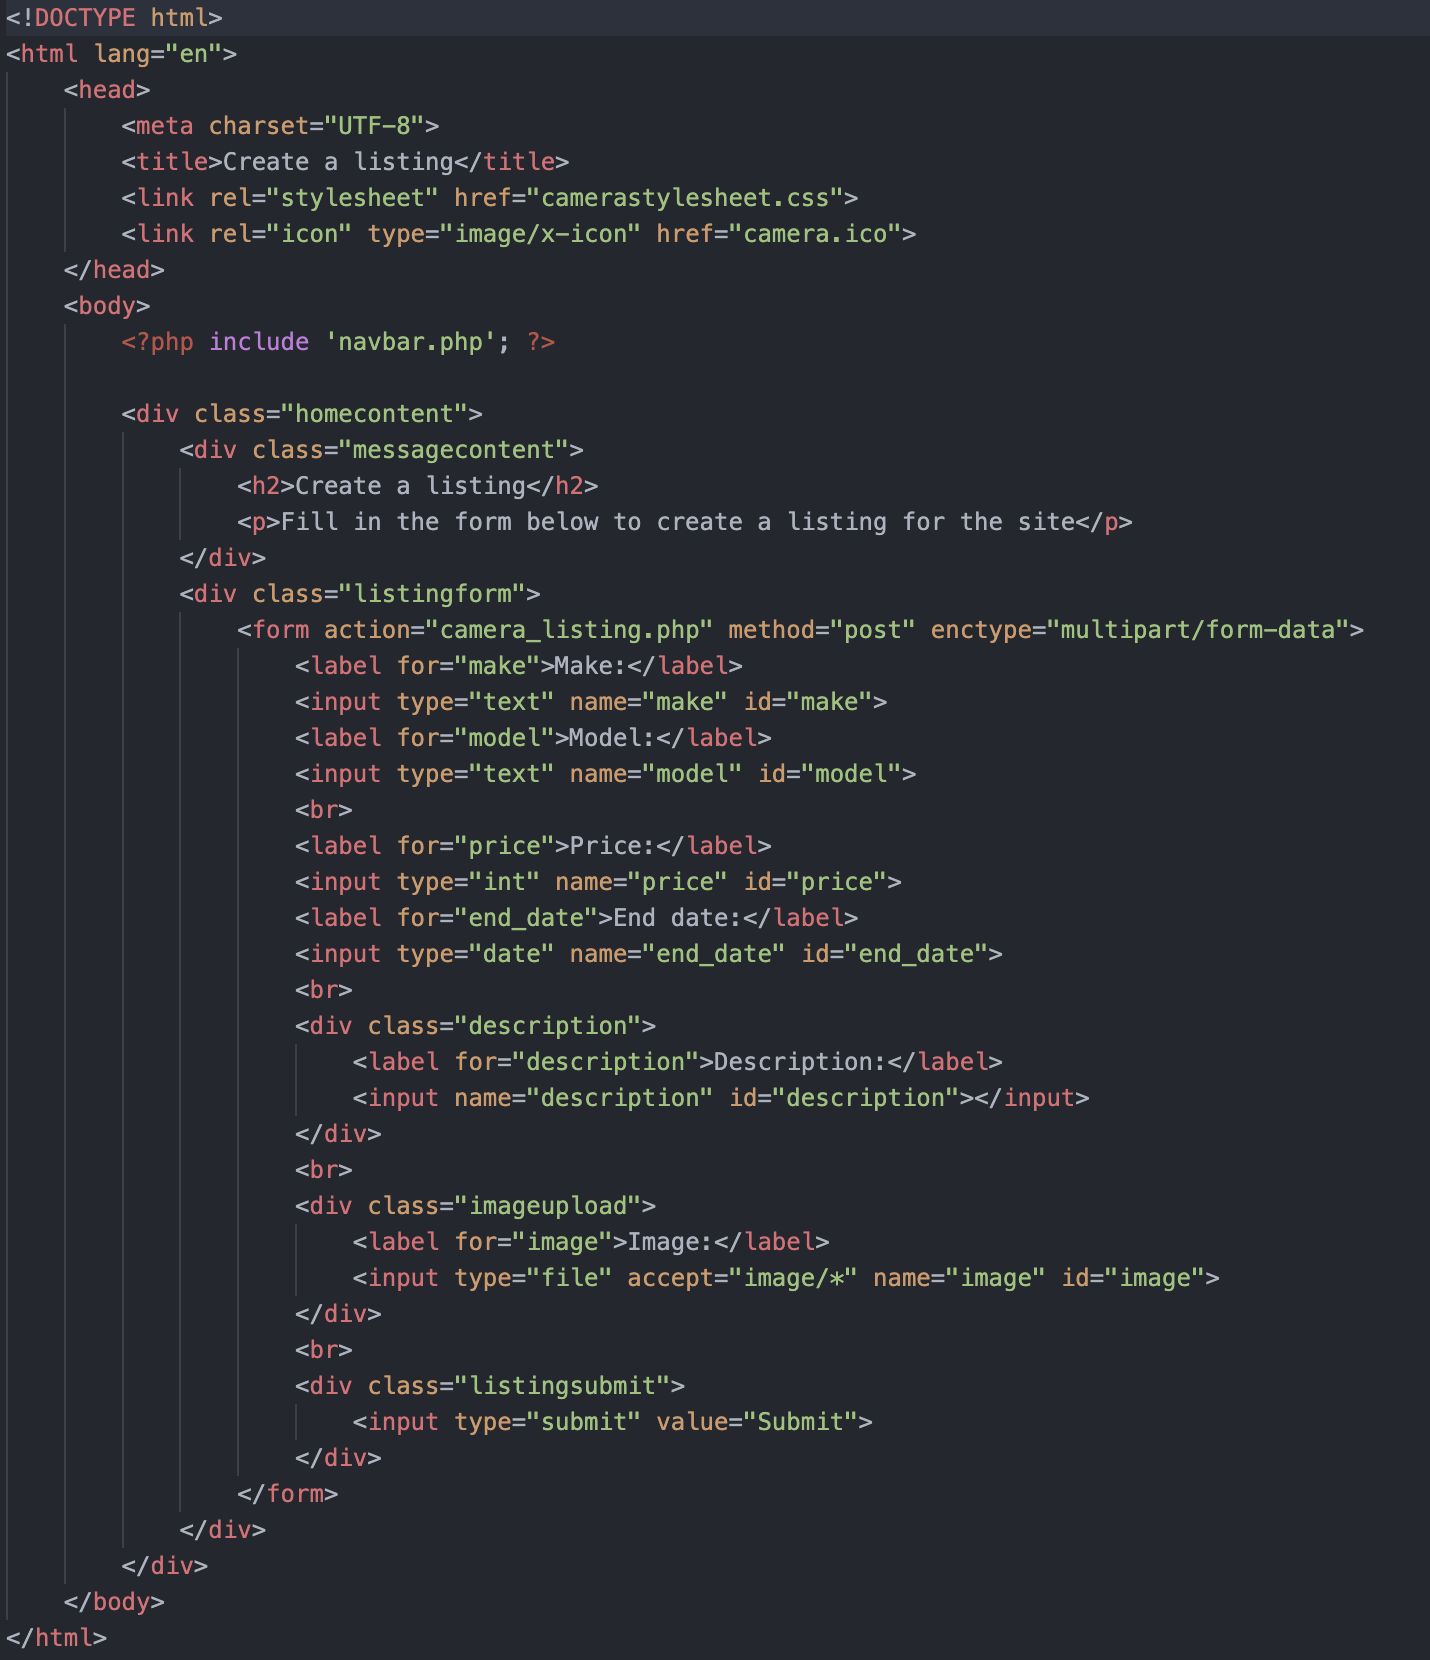
\includegraphics[scale=0.5]{ch3_developing/proto3/createhtml.png}
    \caption{Prototype 3 create a listing HTML code}
    \label{fig:proto3_createhtml}
\end{figure} 
\begin{figure}[H]
    \centering
    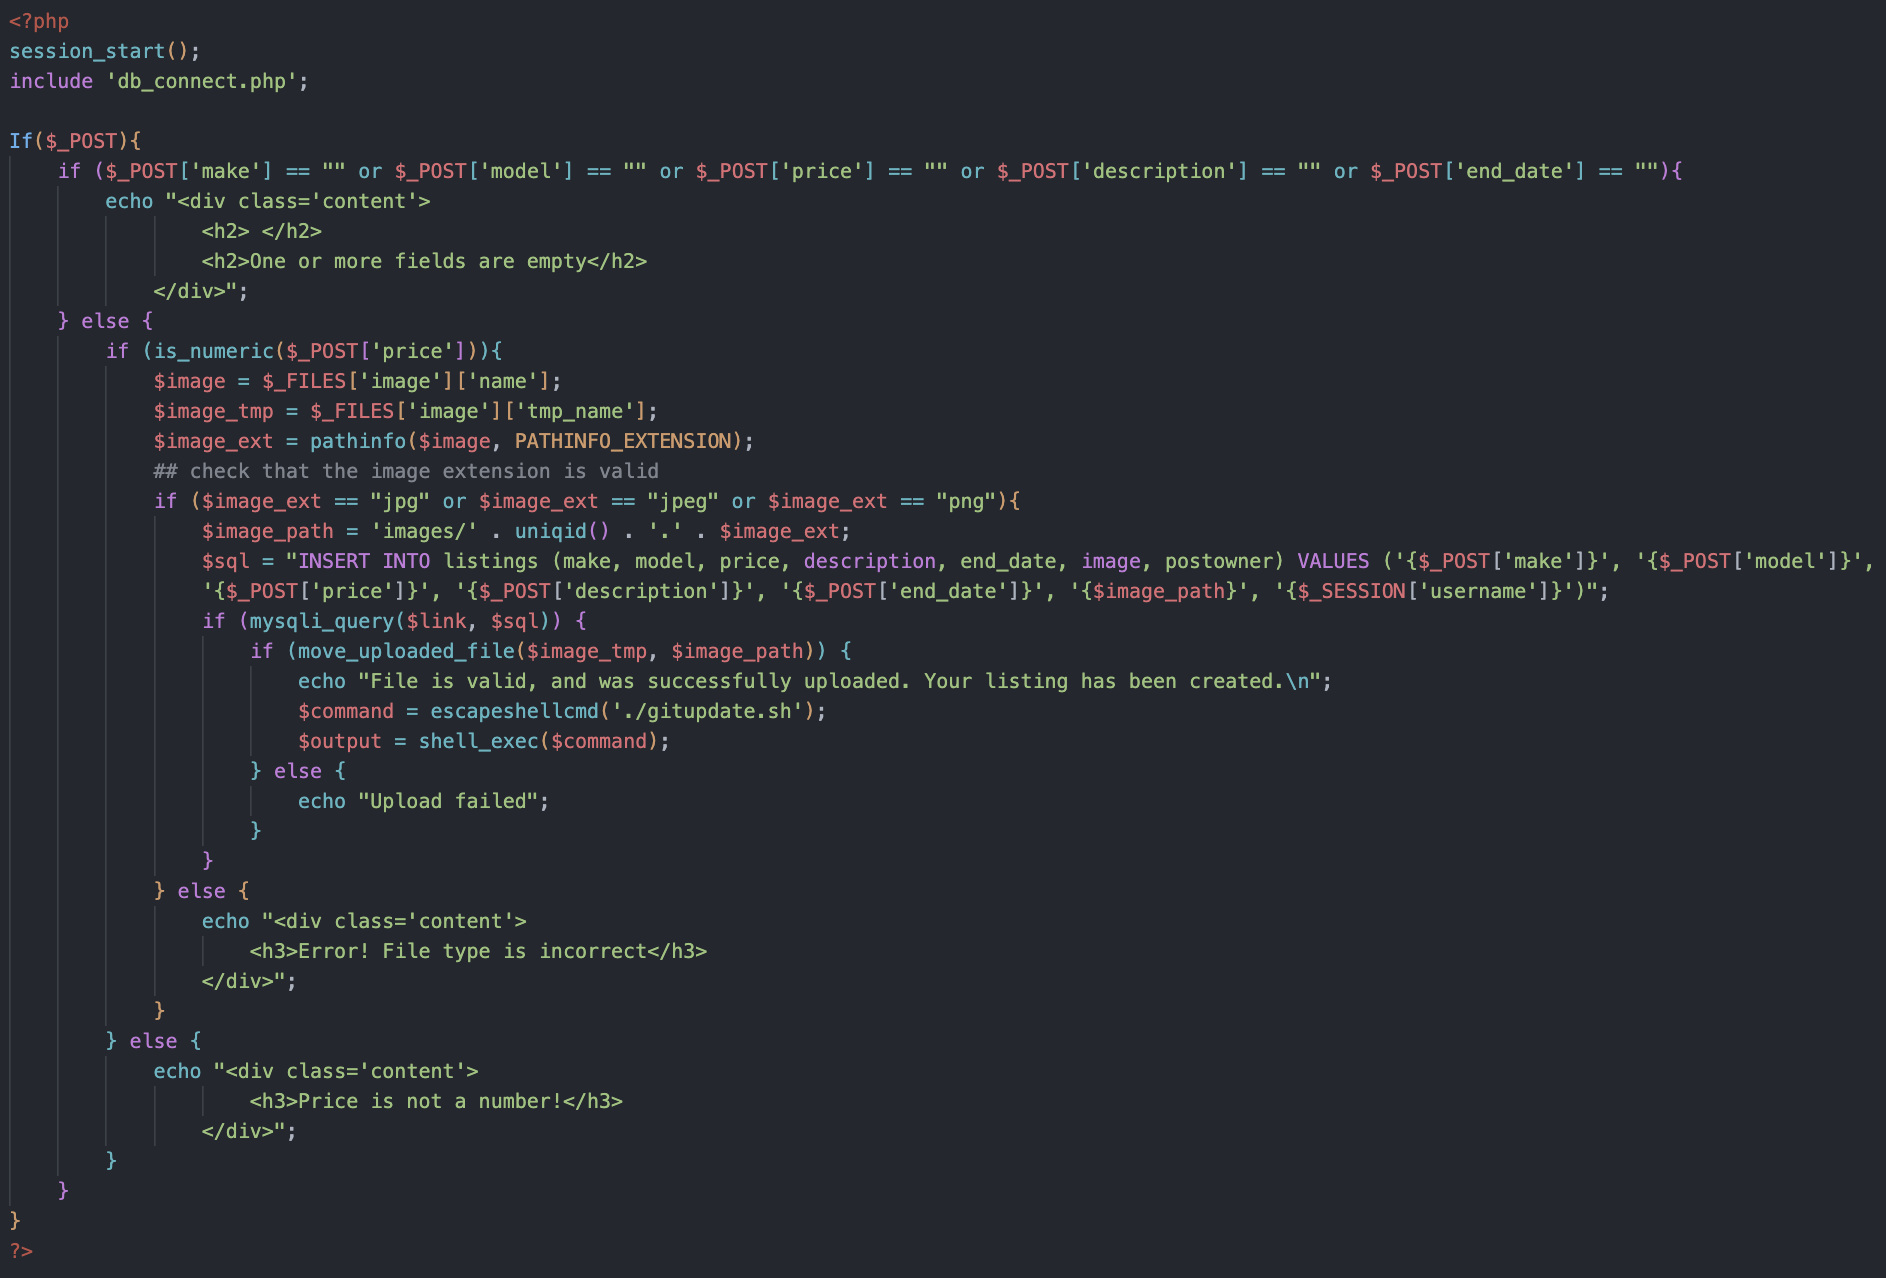
\includegraphics[scale=0.45]{ch3_developing/proto3/create.png}
    \caption{Prototype 3 create a listing code}
    \label{fig:proto3_create}
\end{figure}
The create a listing code has had the addition of more verification for inputs specifically the price and the file extension. The inputs are first all checked to contain something meaning that the rest of the verification processes will work. The price is then checked to only contain numbers, if this is met then the algorithm proceeds to gather the image information and to check that file extension is valid. I chose to only allow 3 file extensions as it covered the majority of images that a user might want to upload. If all tests are passed, then the users listings is added and the image is added to the server. A GitHub script is then ran through the shell to ensure the running of the site. There are error messages corresponding to every point of verification. The HTML code has also been updated in order to only allow the user to upload image files into the image upload section. Whilst operating systems will not enforce this, it does act as another level of verification to stop the user uploading any file for the listing image that is not an actual image.
\subsection{Price recommendation}
 \begin{figure}[H]
    \centering
    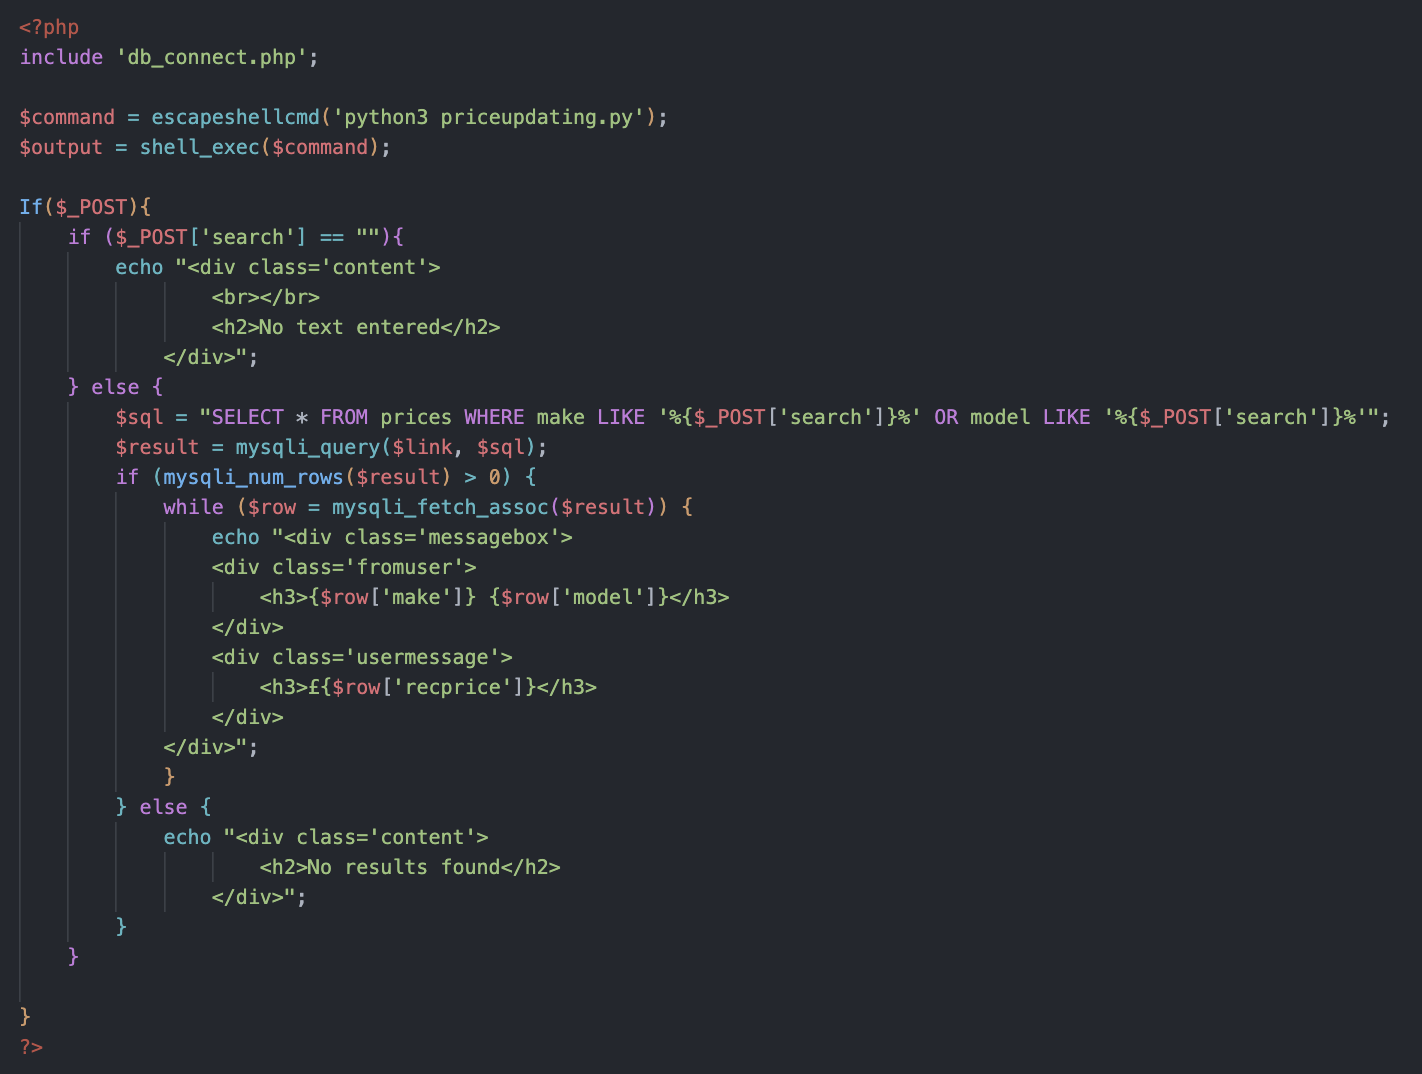
\includegraphics[scale=0.5]{ch3_developing/proto3/recprice.png}
    \caption{Prototype 3 price recommendation}
    \label{fig:proto3_price}
\end{figure}
The price recommendation code works to first run the python price update script shown in Figure 47 through a shell command. This runs on page opening. Once the user has pressed submit, the form is first checked to ensure that it contains text within to ensure that the SQL statement runs correctly. If this is the case, the SQL statement is compiled and ran with the result being echoed with the relevant html to format the code. An error message is shown if the user does not enter text.
\begin{figure}[H]
    \centering
    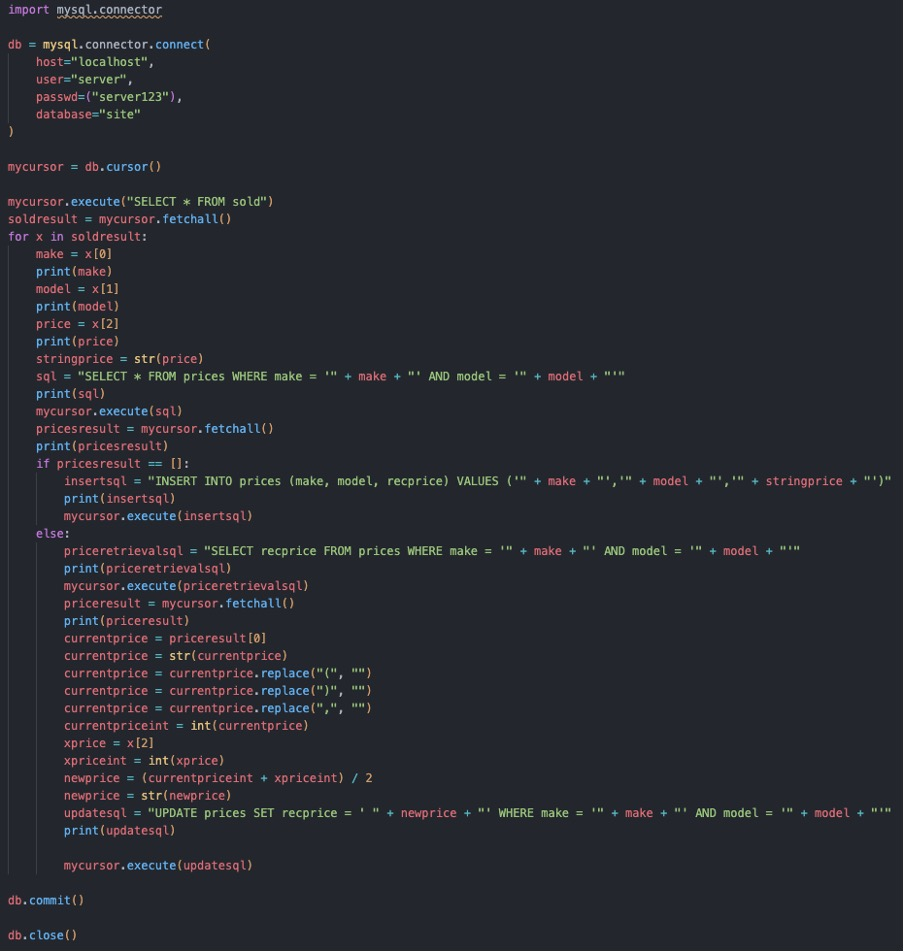
\includegraphics[scale=0.4]{ch3_developing/proto3/pricepython.jpg}
    \caption{Prototype 3 price recommendation python script}
    \label{fig:proto3_pricepython}
\end{figure}
The SQL connector is first imported into python so that SQL queries can be used. We then define the database connection and the connector to make passing SQL statements easier. We then collect all the sold listings from the table. We then cycle through each of the results that are fetched. The make and model are used to query the SQL database under the recommended prices table in order to check whether a recommended price already exists. If no record is found, then we know the make and model have sold on the site for the first time. If this is the case, then we insert the make, model and sold price straight into the database. Else, we fetch the current recommended price in order to update it. The output from the query has to be format and corrected using the replace function in python. After this, the latest sold price and the recommended price are added together and then divided by 2. This creates an average for the recommended price and ensures it is up to date. We then update the record in the recommended price table and close the database connection. 
\subsection{View listing}
\begin{figure}[H]
    \centering
    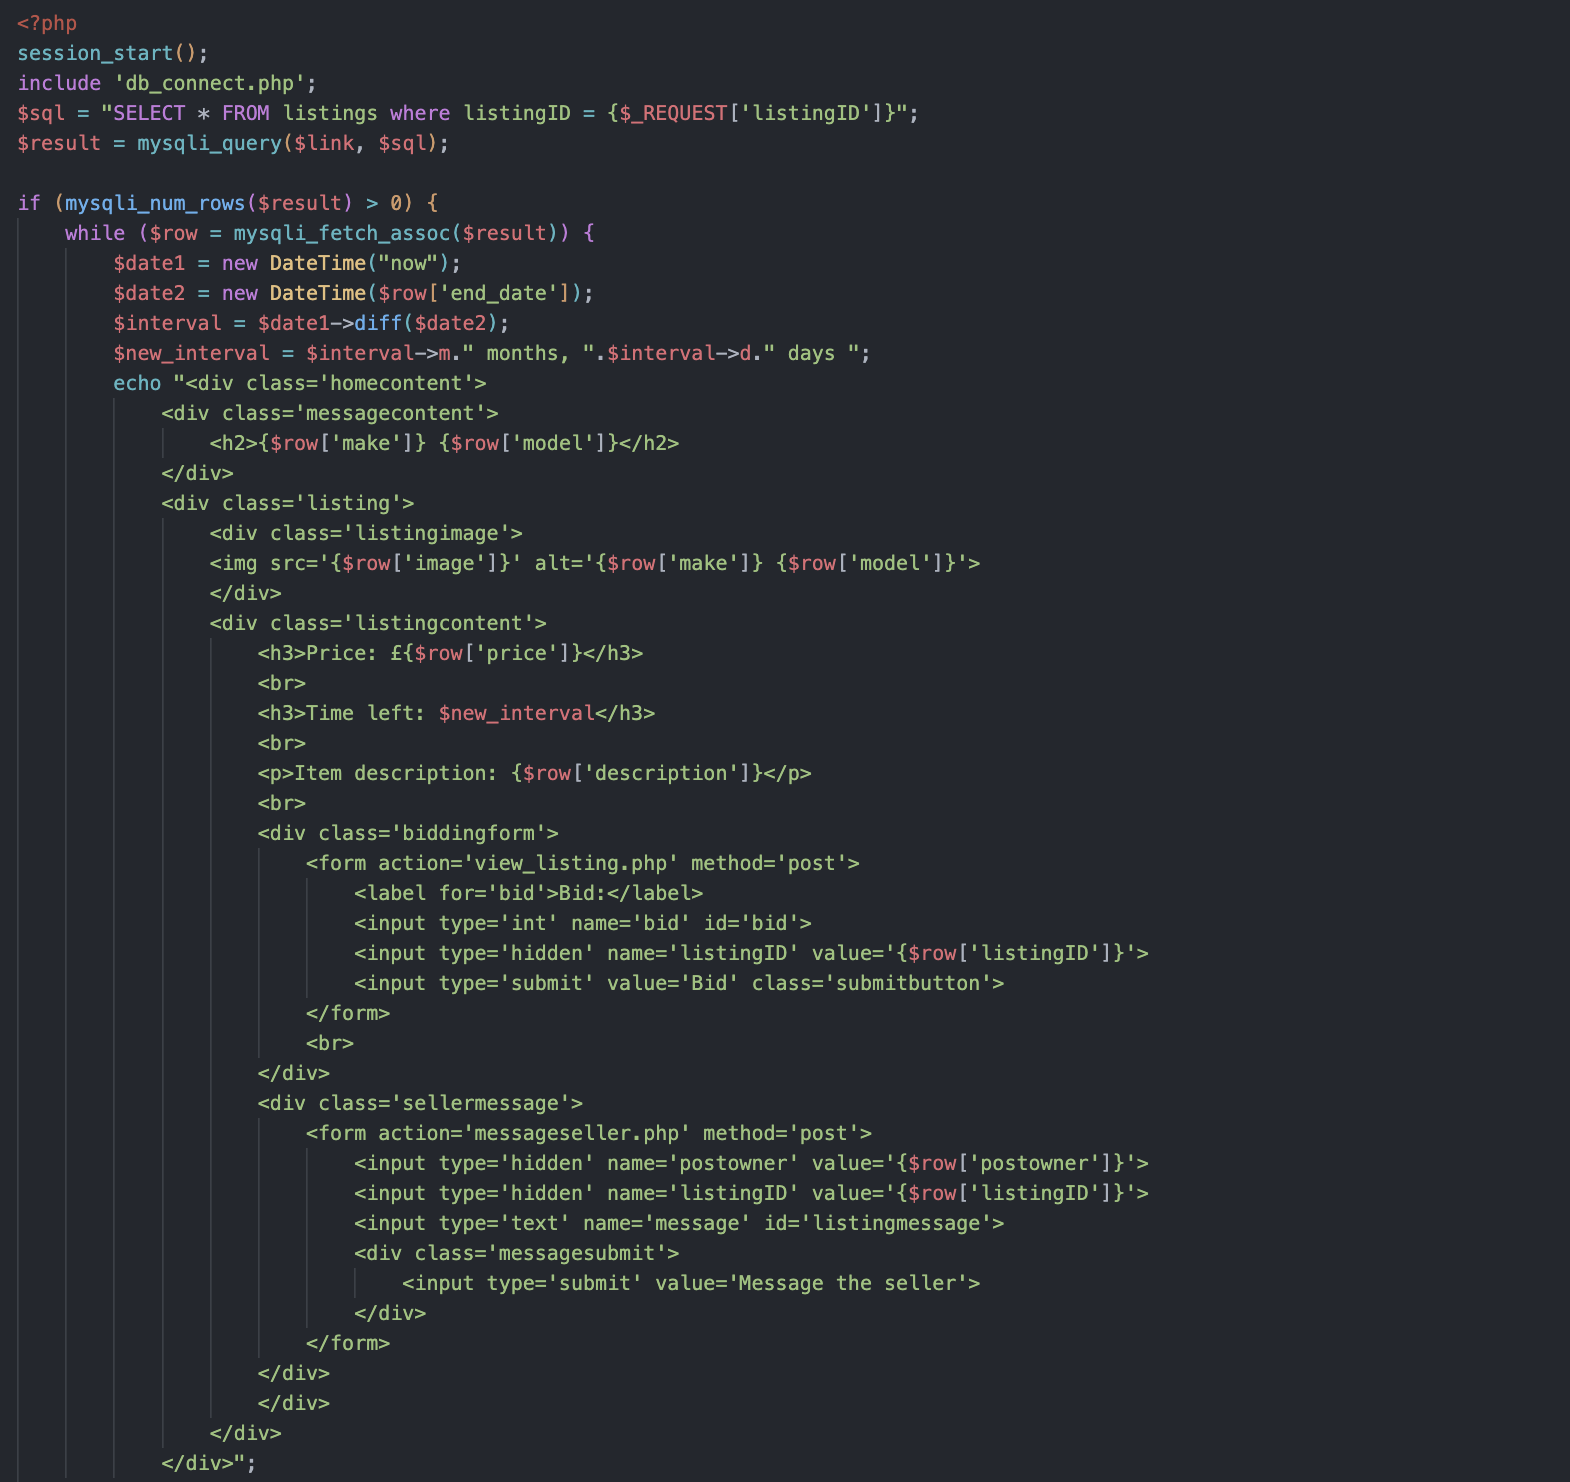
\includegraphics[scale=0.5]{ch3_developing/proto3/view1.png}
    \caption{Prototype 3 view listing code to show the listing}
    \label{fig:proto3_view1}
\end{figure}
This is the view listing code that shows the initial listing from the database. It works by taking the listingID from the search page as a request in the URL bar. The listingID is then used to fetch all the relevant information from the SQL table for that listing. Similar to the search page, the interval has to be calculated in order for the user to see how long is left in an easier format to digest. The listings content is then output through a large echo statement that contains all the information that has been fetched alongside the HTML formatting in order to give the listing its appearance. The bid and message forms are displayed which will allow the user to bid on the item or to send the seller a message. The message box uses the POST format to send the data to the send message PHP page, see \ref{fig:proto3_sendalg}.
\begin{figure}[H]
    \centering
    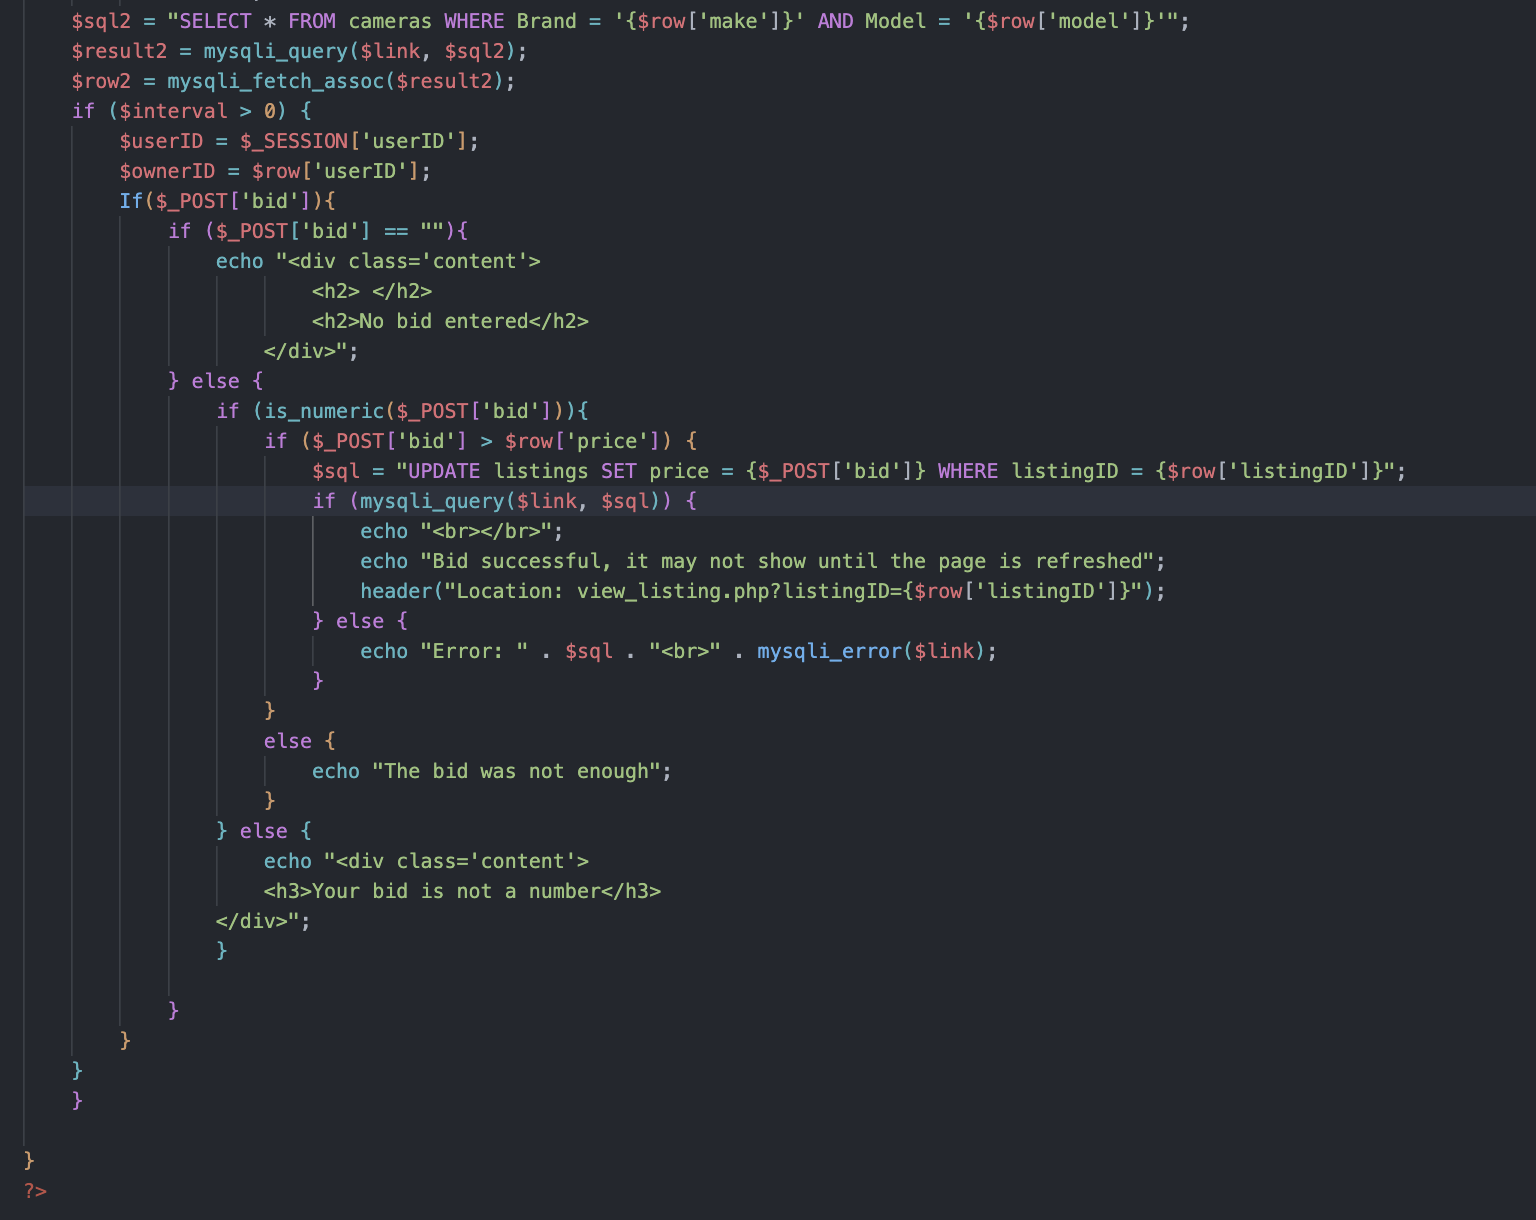
\includegraphics[scale=0.5]{ch3_developing/proto3/view2.png}
    \caption{Prototype 3 view listing code for bidding and messaging}
    \label{fig:proto3_view2}
\end{figure}
This is the view listing PHP code that will verify the bid that they have entered. We first have to check that the user has entered a bid into the box when they’ve submitted. If not, an error is displayed. If they have entered a bid, we then have to check that the bid only contains numbers. This was done after checking the form was blank in order to ensure that the verification that the bid was a number worked without a problem. Providing that the bid contains text and only contains numbers, the bid is then checked that it is greater than the current listing bid. If this condition is met then we update the bid, display a message to say the bid has gone through. In previous prototypes, the page would just be refreshed which caused issues as the url would no longer have the listingID and so the user would have to re-search for the listing. In this prototype, the listingID is now fetched as well, meaning we can redirect the user to the correct page which instantly shows the new bid.

\subsection{Send a message}
 \begin{figure}[H]
    \centering
    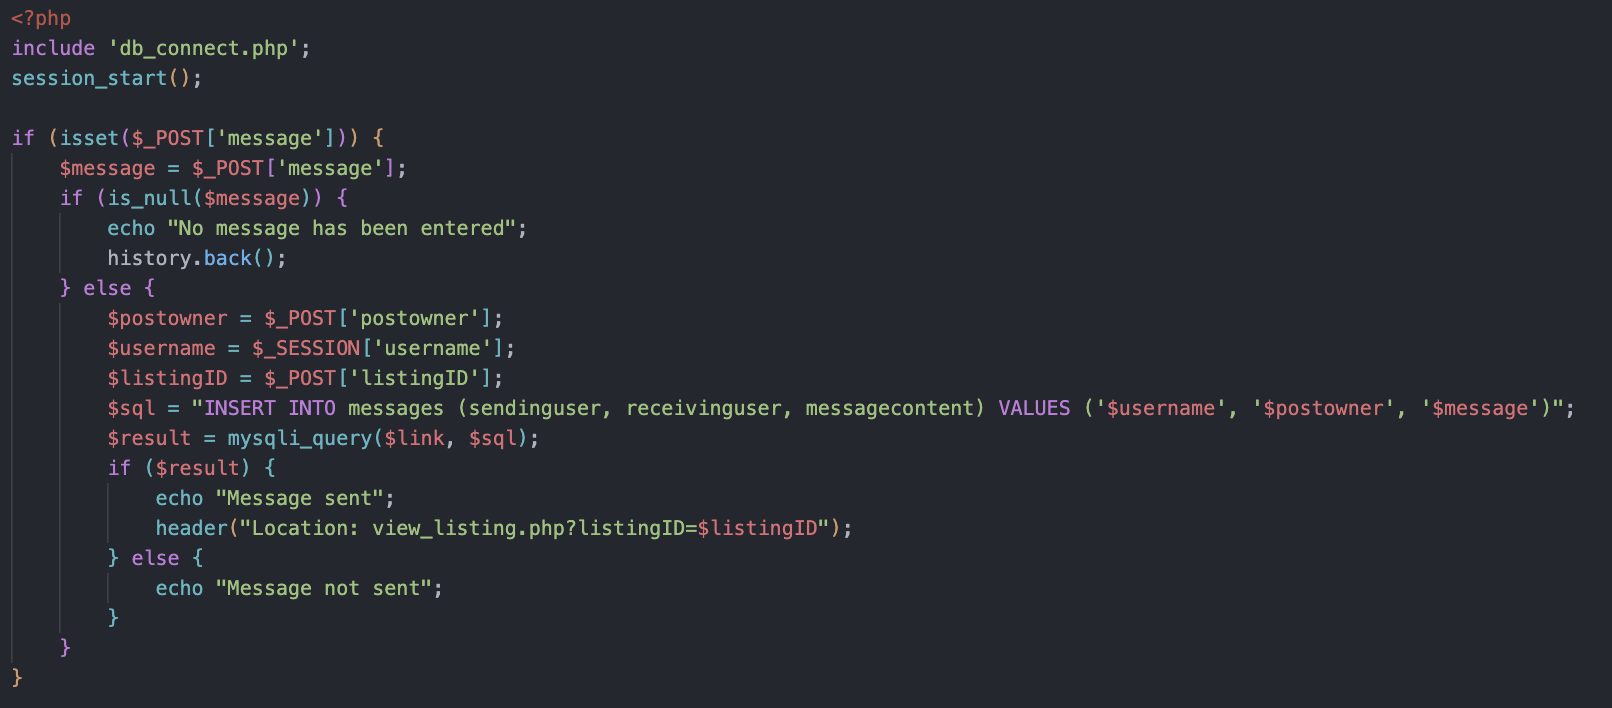
\includegraphics[scale=0.5]{ch3_developing/proto3/messageseller.png}
    \caption{Prototype 3 send message code}
    \label{fig:proto3_sendmessagecode}
\end{figure}
The send message code will run when the user presses submit on the send message button on the view listing page. It first collects the message from the form and checks that the message is not empty. This has been achieved with the is\_null() function within PHP. If the message is empty, the user is given an error and then send back to the view listing page. Else, the postowner and listingID is collected from the form. The postowner is collected from the listing as we need to know the recipient of the messages. The username is also collected in order to add a sending user. It is fetched using a session variable. The message is then complied and executed in the SQL statement. If the SQL statement goes through without a problem, then the user is sent back to the listing that they were viewing. This is why we had to collect the listingID from the form on the view listing page. If there are any issues with the SQL statement, the user is given an error saying the message was not sent. 
\subsection{View messages}
  \begin{figure}[H]
    \centering
    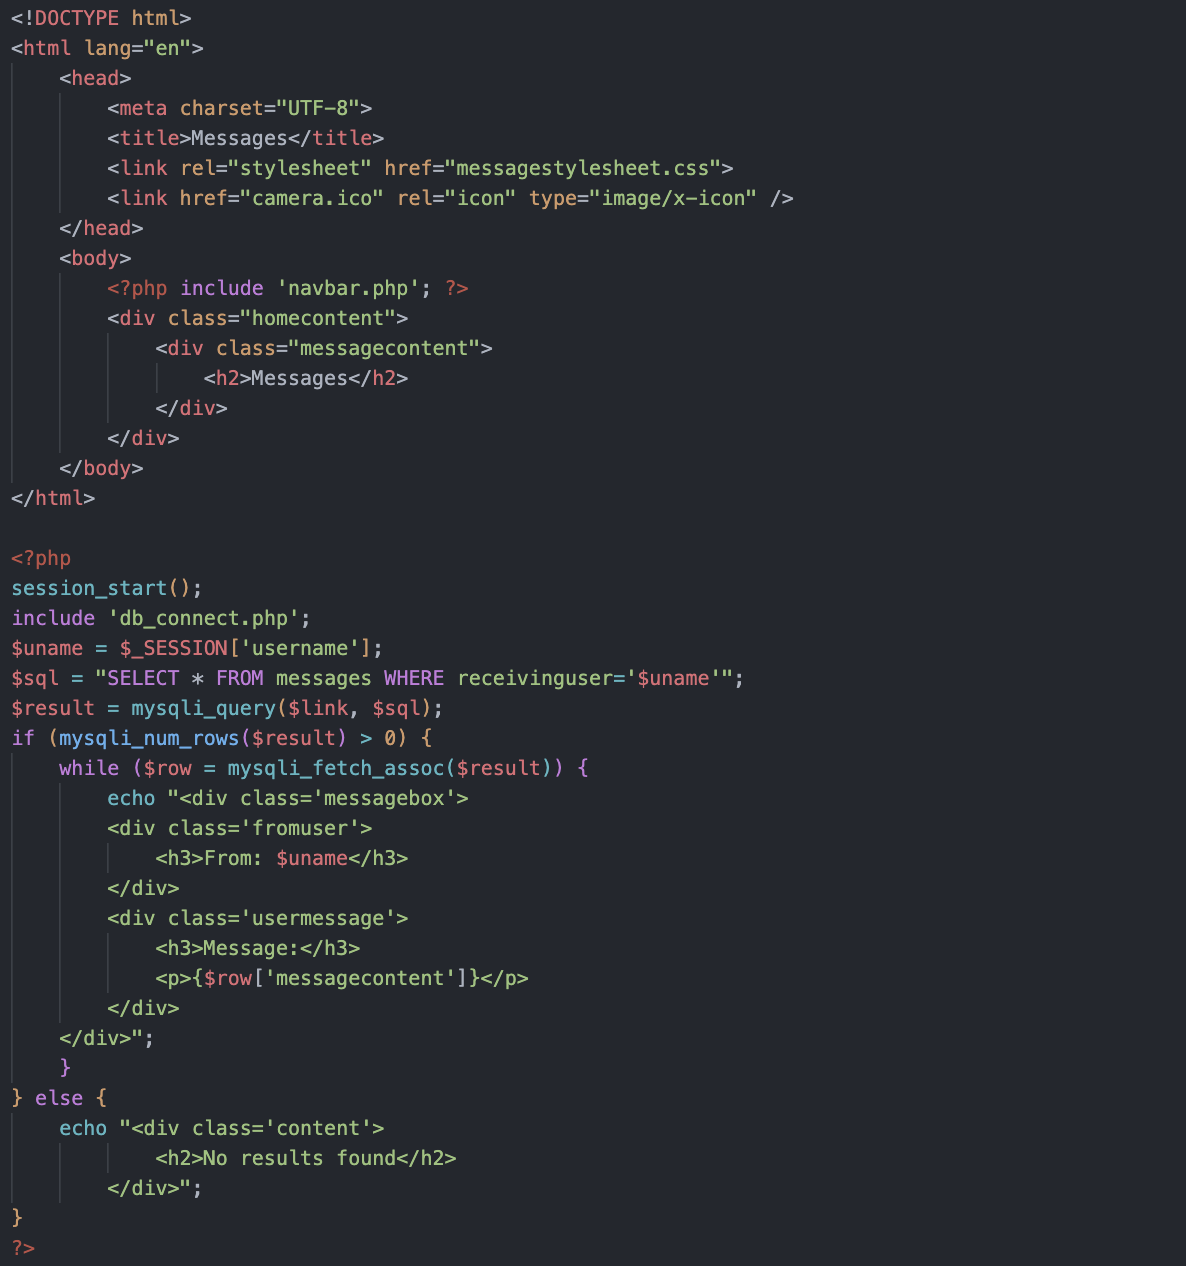
\includegraphics[scale=0.6]{ch3_developing/proto3/messages.png}
    \caption{Prototype 3 view messages code}
    \label{fig:proto3_viewmessage}
\end{figure}
This is the code that will process and collect the messages for the user. The messages are stored in a table within the database. When the user opens the page, their username is collected from the session variable. It is then used to query the database for all the messages that the user has received. We then use a while loop to cycle through the messages and output one with the relevant html for formatting. An error message is displayed if no messages are found.

\subsection{Testing}
\begin{center}
\begin{longtable}{|P{17mm}|P{17mm}|P{16mm}|P{17mm}|P{60mm}|}
  \hline
  \textbf{Test} & \textbf{Type} & \textbf{Expected result} & \textbf{Actual result} & \textbf{Test evidence} \\
  \hline
  \endfirsthead
  \hline
  \endhead
  \hline 

  \endfoot
  \endlastfoot
Signup page displays register form & Normal & Form is displayed &
Pass -- as expected &
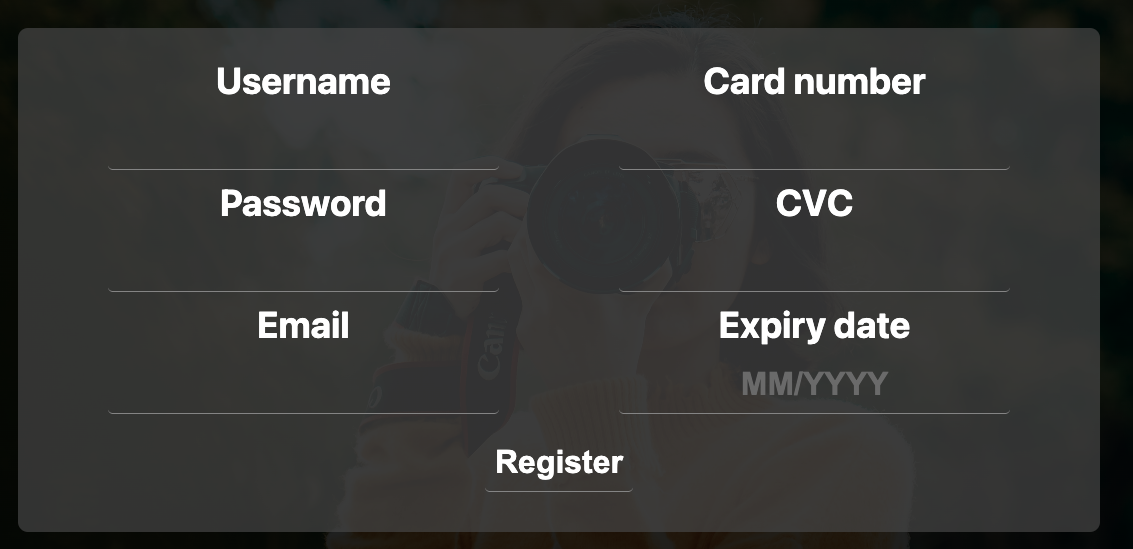
\includegraphics[width=58mm]{ch3_developing/proto3/media/image2.png} \\ \hline
Form is blank & Erroneous & Error message displayed & Pass -- as
expected &

\includegraphics[width=58mm]{ch3_developing/proto3/media/image3.png} \\ \hline
Card number or cvc is not text & Erroneous & Form only allows number
input & Pass -- as expected &
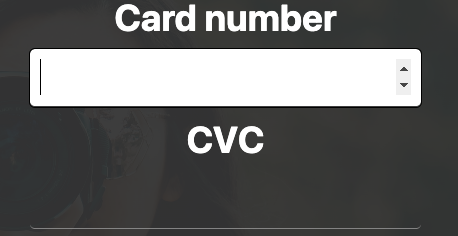
\includegraphics[width=58mm]{ch3_developing/proto3/media/image4.png} \\ \hline
Card number not long enough & Erroneous & Error message to user & Pass
-- as expected &
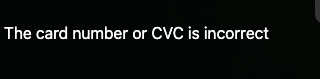
\includegraphics[width=58mm]{ch3_developing/proto3/media/image5.png} \\ \hline
CVC not long enough & Erroneous & Error message displayed & Pass -- as
expected &
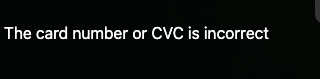
\includegraphics[width=58mm]{ch3_developing/proto3/media/image5.png} \\ \hline
Details entered correctly & Normal & Details to database and user
forwarded to home page & Pass -- forwarded to home page &
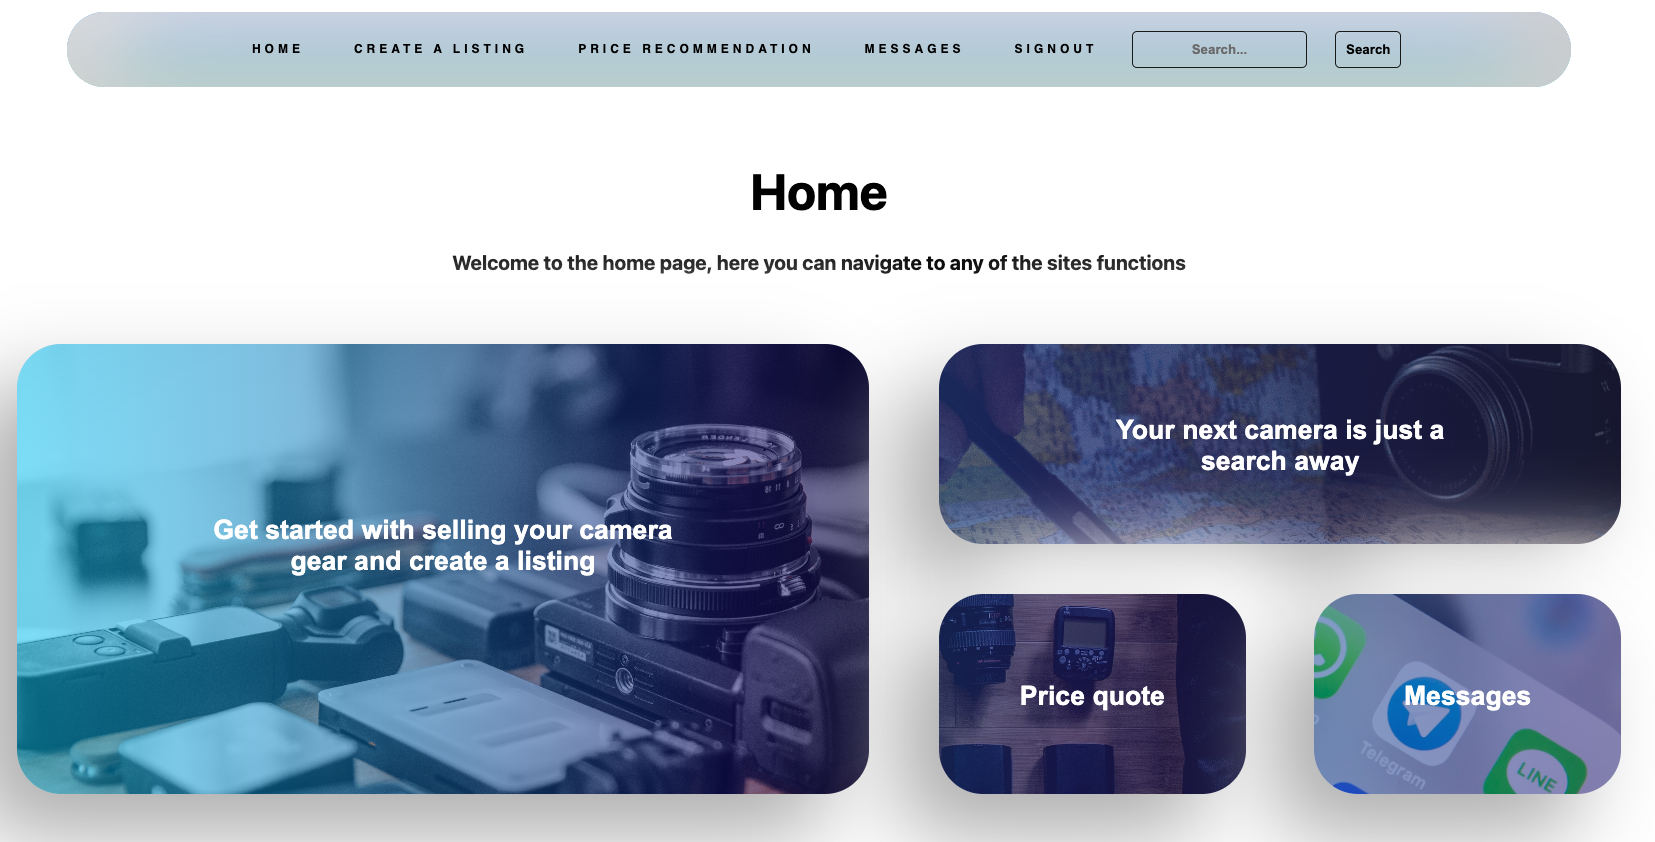
\includegraphics[width=58mm]{ch3_developing/proto3/media/image6.png} \\ \hline
Signup details are hashed & Normal & Details in database are
hashed & Pass -- all inputs are hashed &
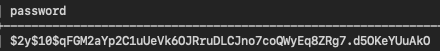
\includegraphics[width=58mm]{ch3_developing/proto3/media/image7.png}

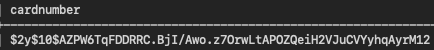
\includegraphics[width=58mm]{ch3_developing/proto3/media/image8.png}

All are hashed with two columns shown \\ \hline
Login page displays form & Normal & Form is displayed to user & Pass --
form is shown &
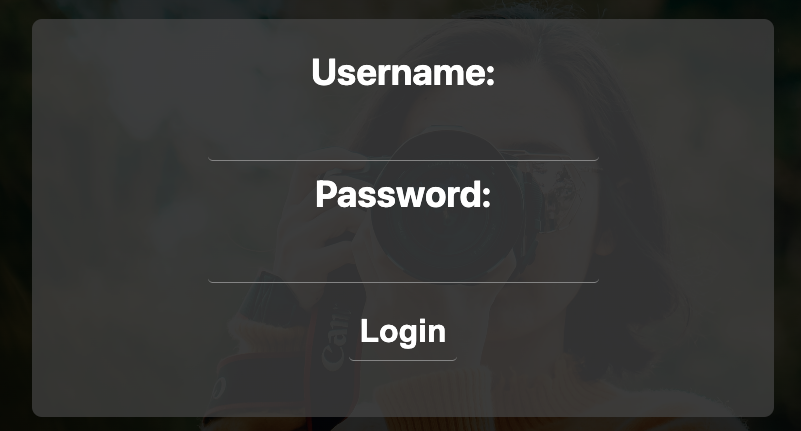
\includegraphics[width=58mm]{ch3_developing/proto3/media/image9.png} \\ \hline
Login form is submitted blank & Erroneous & Error message shown to user
& Pass -- message shown &

\includegraphics[width=58mm]{ch3_developing/proto3/media/image10.png} \\ \hline
Login page contains forgot password button & Normal & Button is shown &
Fail & Feature not built due to time \\ \hline
User is shown form to enter username and email & Normal & The user has a
2-text box form displayed & Fail & Feature not built due to time \\ \hline
If username and password match user is sent & Normal & The user is sent
an email with a replacement password & Fail & Feature not built due to
time \\ \hline
User is given an error is they do not match & Erroneous & The user is
shown an error & Fail & Feature not built due to time \\ \hline
User is shown an error if the forms are blank & Erroneous & The user is
shown an error & Fail & Feature not built due to time \\ \hline
Correct details forwards user to home page & Normal & User is forwarded
to the homepage & Pass -- home page displayed &
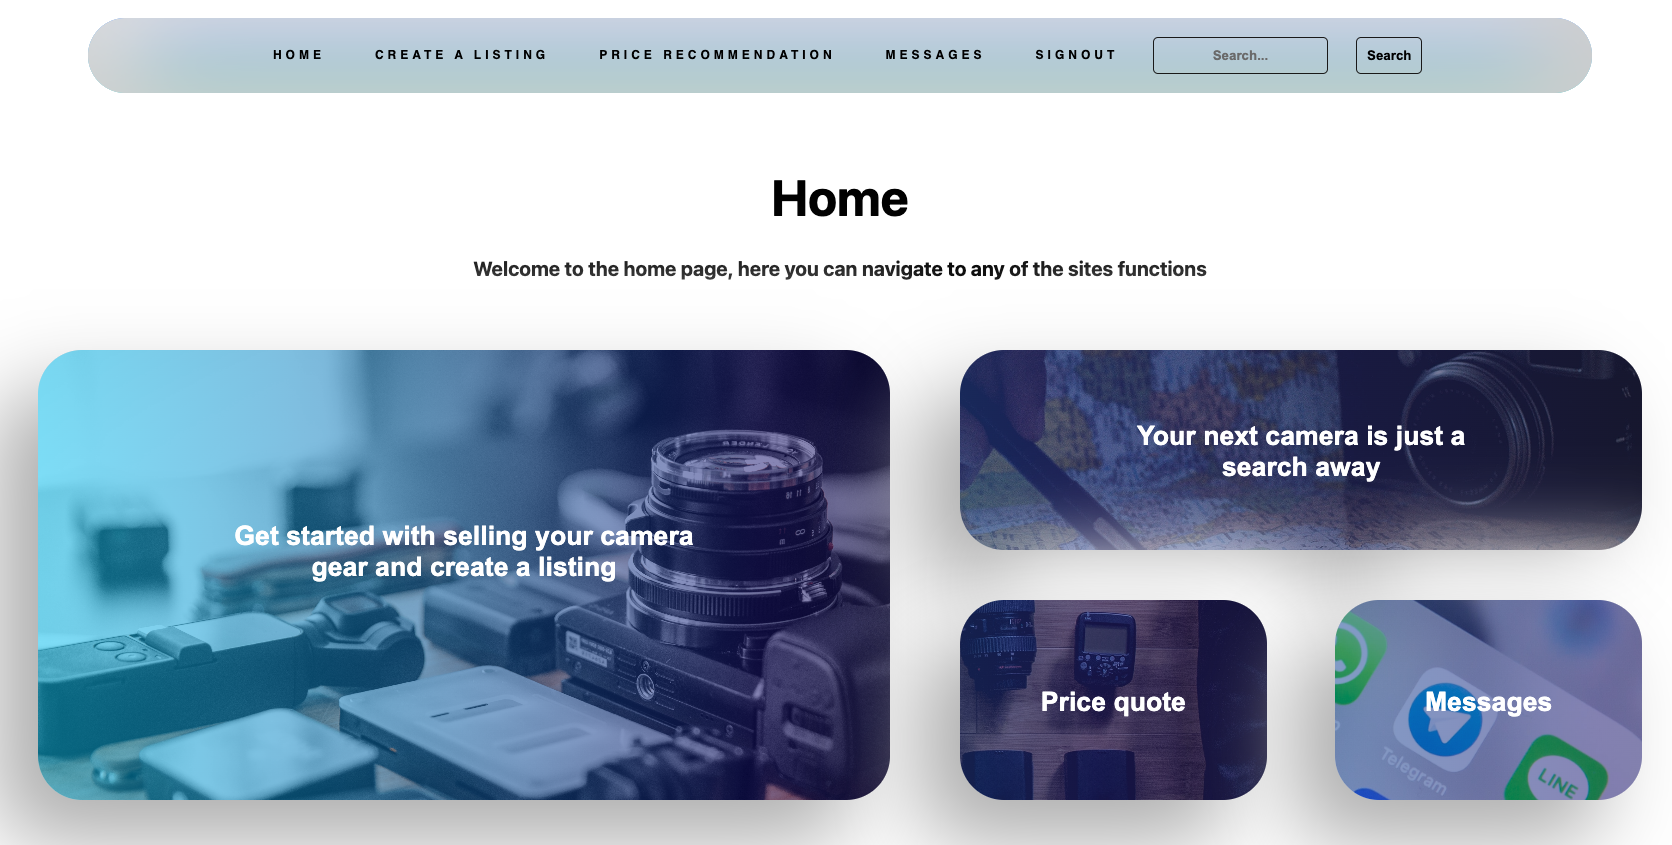
\includegraphics[width=58mm]{ch3_developing/proto3/media/image11.png} \\ \hline
User enters incorrect details & Erroneous & Details incorrect message &
Pass -- as expected &

\includegraphics[width=58mm]{ch3_developing/proto3/media/image12.png} \\ \hline
Home page displays navigation bar & Normal & Bar displayed at top of
screen & Pass -- as expected &
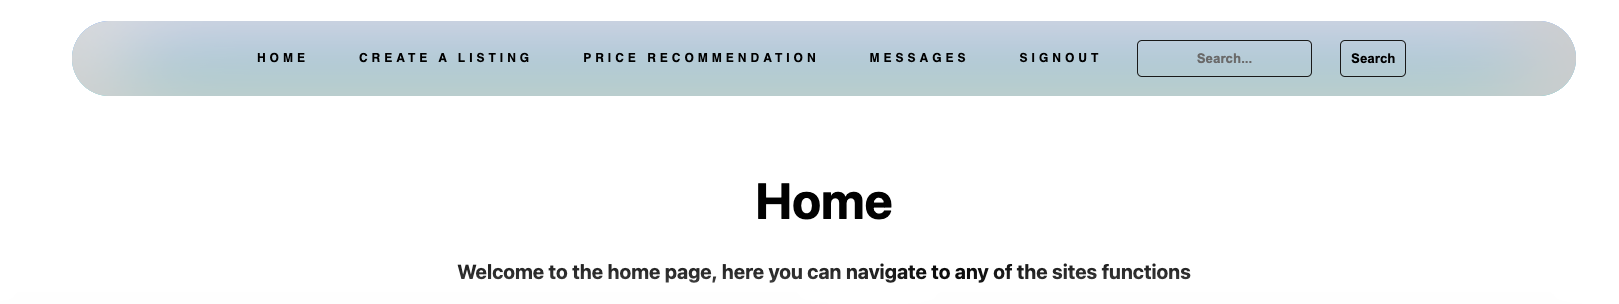
\includegraphics[width=58mm]{ch3_developing/proto3/media/image13.png} \\ \hline
Home page displays 4 buttons for each page & Normal & Buttons on
homepage with image & Pass -- as expected &
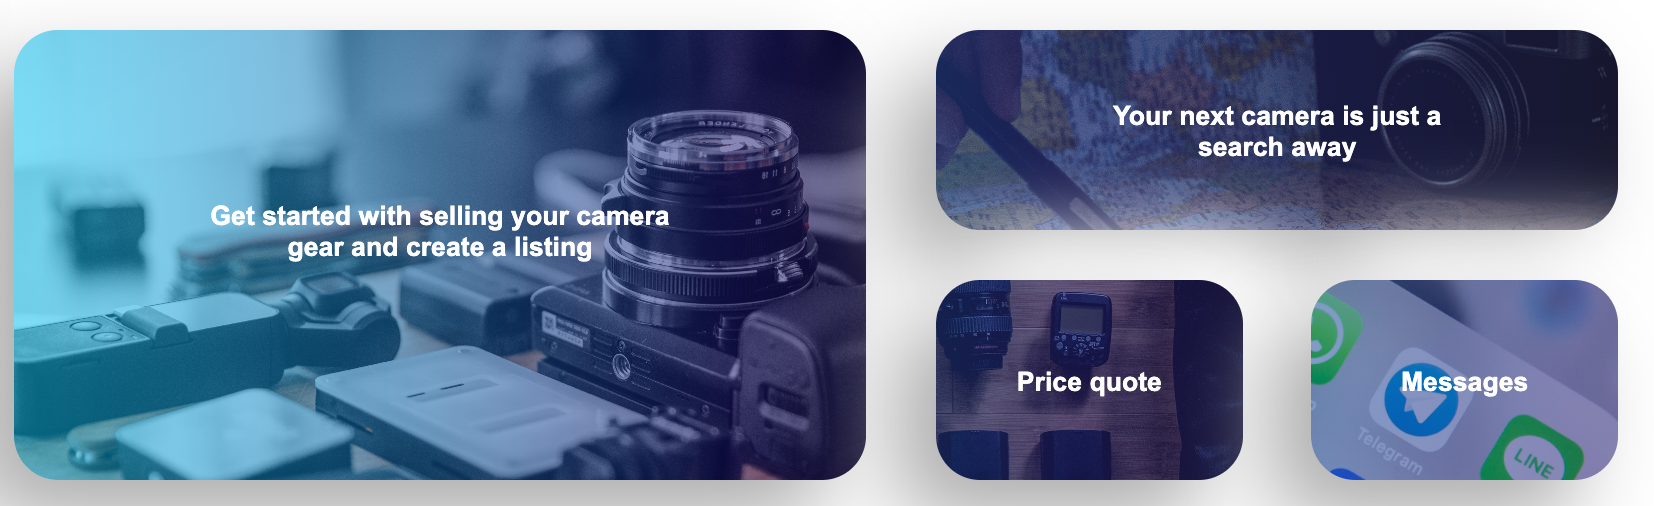
\includegraphics[width=58mm]{ch3_developing/proto3/media/image14.png} \\ \hline
Create a listing page displays form & Normal & Form shown to user & Pass
-- form is displayed &
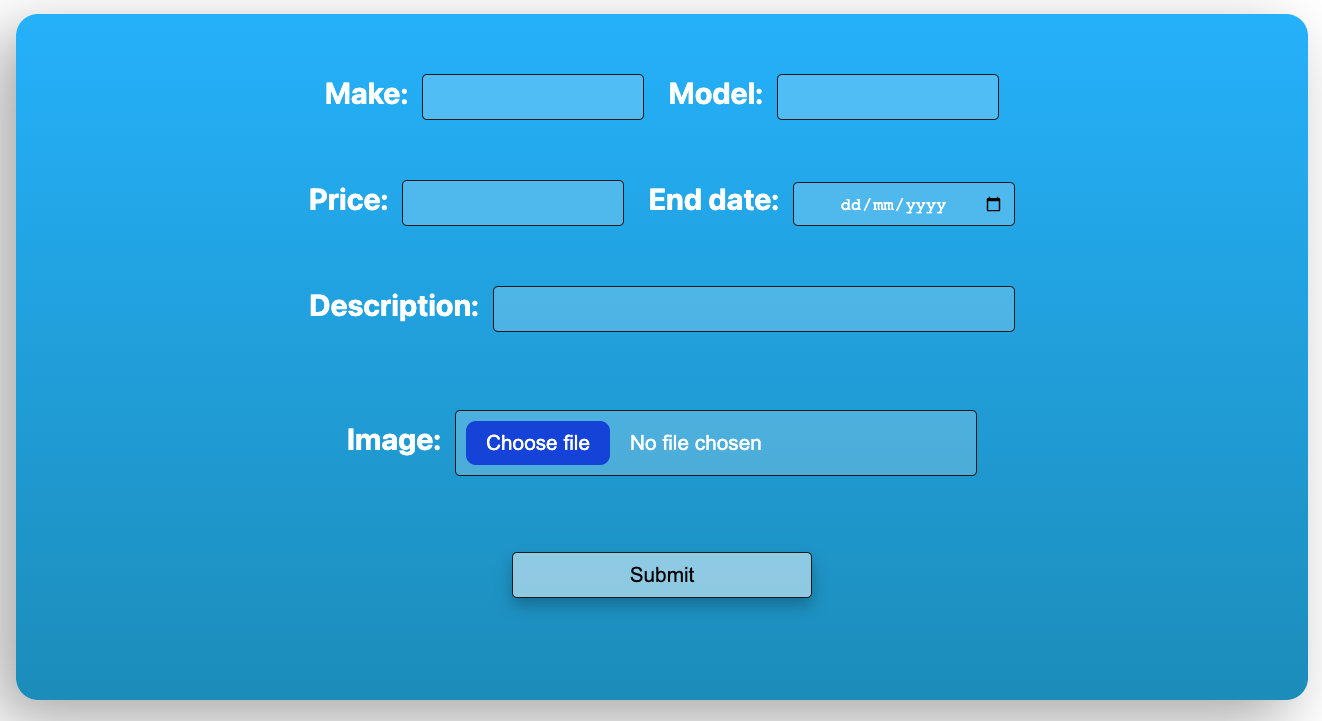
\includegraphics[width=58mm]{ch3_developing/proto3/media/image15.png} \\ \hline
Create a listing form allows text entry & Normal & User can input text
and file & Pass -- as expected &
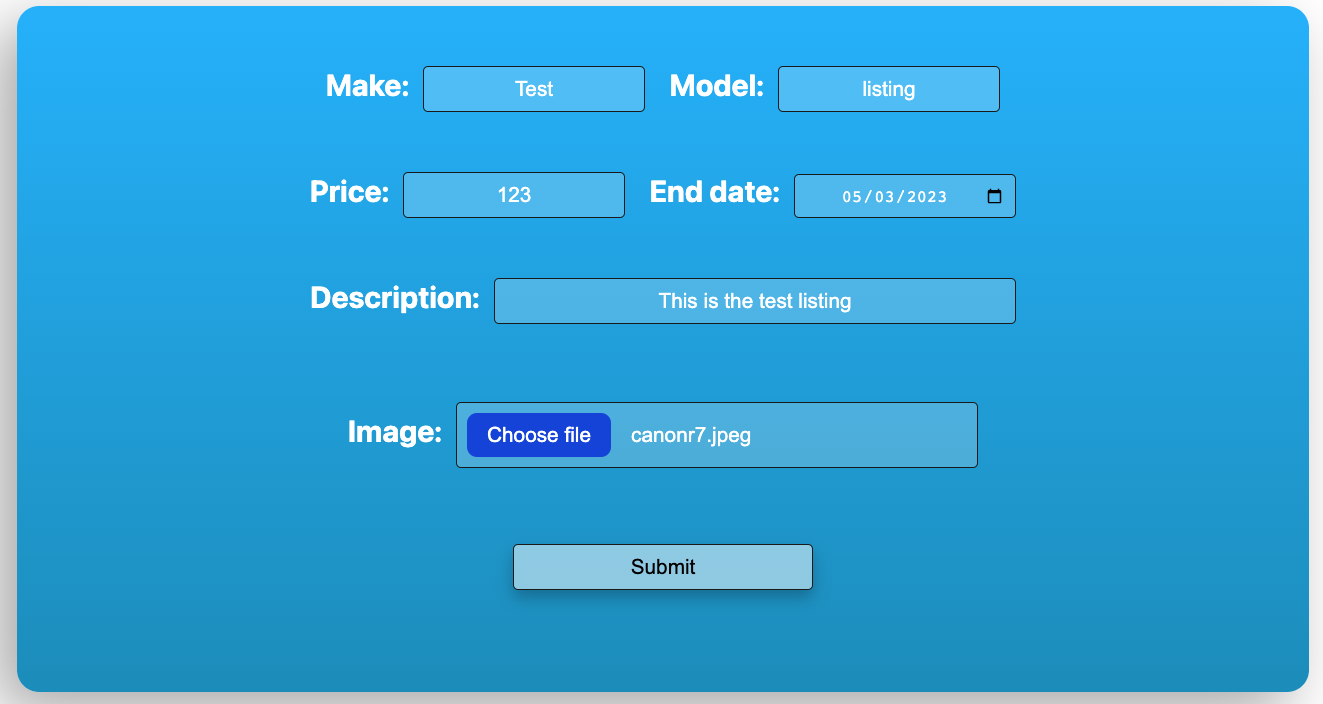
\includegraphics[width=58mm]{ch3_developing/proto3/media/image16.png} \\ \hline
Submitting a normal listing & Normal & Listing is sent to database &
Pass -- as expected &

\includegraphics[width=58mm]{ch3_developing/proto3/media/image17.png}

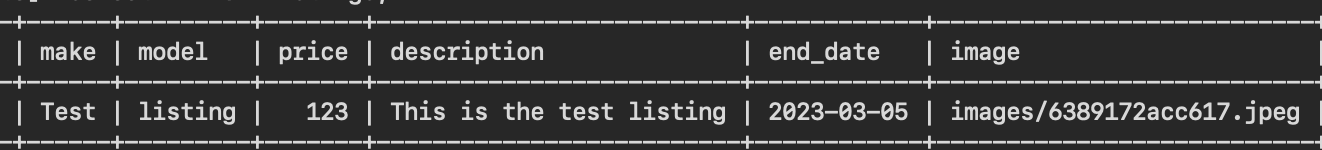
\includegraphics[width=58mm]{ch3_developing/proto3/media/image18.png} \\ \hline
Listing price is not a number & Boundary & Error message displayed &
Pass -- as expected &

\includegraphics[width=58mm]{ch3_developing/proto3/media/image19.png} \\ \hline
Create listing form is submitted blank & Boundary & Error message shown
& Pass- as expected &

\includegraphics[width=58mm]{ch3_developing/proto3/media/image20.png} \\ \hline
Attempt to upload non-image file & Boundary & Not accepted file type
error & Pass -- message shown &
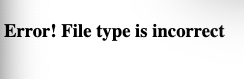
\includegraphics[width=58mm]{ch3_developing/proto3/media/image21.png} \\ \hline
Navigation search bar searches listings & Normal & Search page with
search term loaded & Pass -- as expected &

\includegraphics[width=58mm]{ch3_developing/proto3/media/image22.png}

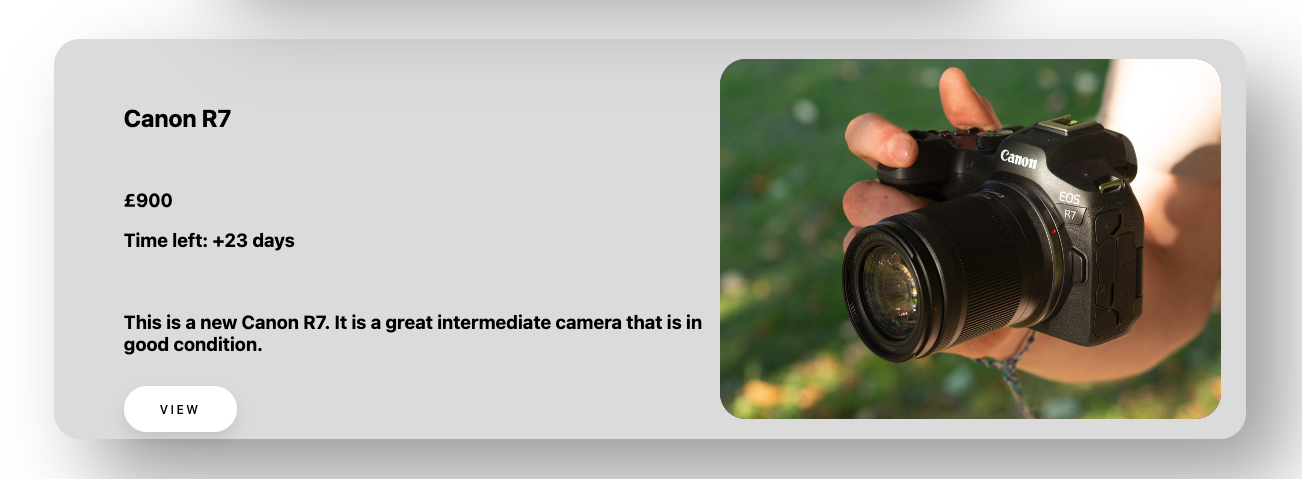
\includegraphics[width=58mm]{ch3_developing/proto3/media/image23.png} \\ \hline
Search box is displayed on search page & Normal & Search box on page &
Pass -- box displayed &
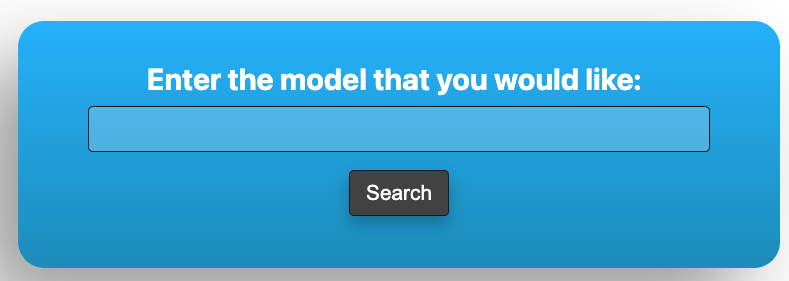
\includegraphics[width=58mm]{ch3_developing/proto3/media/image24.png} \\ \hline
Search box shows listing from search term & Normal & Listing is
displayed & Pass -- listing found &
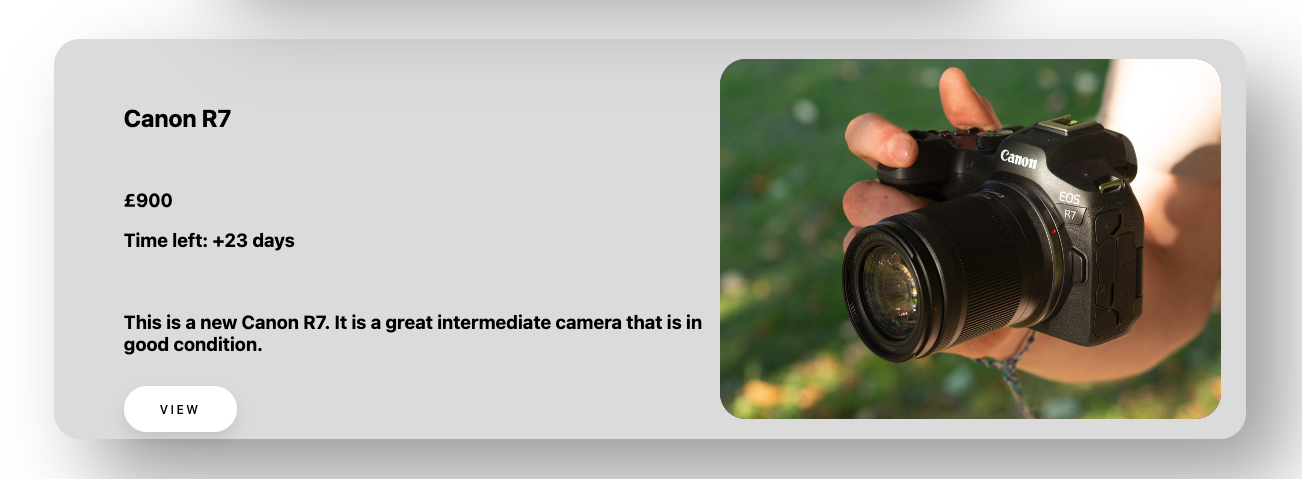
\includegraphics[width=58mm]{ch3_developing/proto3/media/image23.png} \\ \hline
Search box finds no results & Normal & No results found message & Pass
-- as expected &
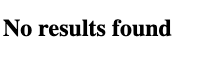
\includegraphics[width=58mm]{ch3_developing/proto3/media/image25.png} \\ \hline
Search box has long search term & Boundary & Works as normal & Pass --
no change &
\includegraphics[width=58mm]{ch3_developing/proto3/media/image26.png}

\includegraphics[width=58mm]{ch3_developing/proto3/media/image27.png} \\ \hline
View listing button takes user to listing page & Normal & User forwarded
to listings specific page & Pass -- listing is shown &
\includegraphics[width=58mm]{ch3_developing/proto3/media/image28.png} \\ \hline
All listing information is displayed & Normal & All information for a
specific listing is shown & Pass -- all information is shown &
\includegraphics[width=58mm]{ch3_developing/proto3/media/image28.png} \\ \hline
Camera information shown & Normal & Camera information from table
displayed & Fail -- No information shown & Feature has not been built
due to time \\ \hline
Bid entered normally & Normal & Bid is processed and updated & Pass --
bid is updated &
\includegraphics[width=58mm]{ch3_developing/proto3/media/image29.png} \\ \hline
Bid is not entered & Erroneous & Error is shown & Fail -- no error shown
&
\includegraphics[width=58mm]{ch3_developing/proto3/media/image28.png} \\ \hline
Bid is not enough & Erroneous & Error is displayed & Pass -- as expected
&
\includegraphics[width=58mm]{ch3_developing/proto3/media/image30.png} \\ \hline
Large bid entered & Boundary & Function runs normally & Pass -- bid
processed &
\includegraphics[width=58mm]{ch3_developing/proto3/media/image31.png} \\ \hline
Message can be entered & Normal & Text can be entered into the message
box & Pass -- as expected &
\includegraphics[width=58mm]{ch3_developing/proto3/media/image32.png} \\ \hline
Message can be sent to seller & Normal & Message processed and then can
be retrieved & Pass -- message shown on messages page &
\includegraphics[width=58mm]{ch3_developing/proto3/media/image33.png} \\ \hline
No message entered & Erroneous & Error shown to user & Fail -- Message
is processed with empty message shown &
\includegraphics[width=58mm]{ch3_developing/proto3/media/image34.png} \\ \hline
Messages are retrieved & Normal & Messages are shown when message page
loaded & Pass -- all messages retrieved &
\includegraphics[width=58mm]{ch3_developing/proto3/media/image35.png} \\ \hline
Price recommendation page shows text box & Normal & Box displayed on the
webpage & Pass -- box shown &
\includegraphics[width=58mm]{ch3_developing/proto3/media/image36.png} \\ \hline
User can type in price recommendation box & Normal & User is able to
enter text & Pass -- user can type &
\includegraphics[width=58mm]{ch3_developing/proto3/media/image37.png} \\ \hline
No text is entered into box & Erroneous & Error is displayed to the user
& Pass -- error displayed &
\includegraphics[width=58mm]{ch3_developing/proto3/media/image38.png} \\ \hline
Price recommendation is fetched & Normal & Price recommendation is
displayed to the user & Pass -- Information displayed &
\includegraphics[width=58mm]{ch3_developing/proto3/media/image39.png} \\ \hline
Price recommendation updated on page run & Normal & D3500 price will
change if code is ran & Pass -- price is updated &
\includegraphics[width=58mm]{ch3_developing/proto3/media/image40.png} \\ \hline

    \caption{Prototype 3 testing table}
\label{tab:proto3_testing}
\end{longtable}
\end{center}
